\documentclass[12pt]{article}

\usepackage[margin=1in]{geometry}
\usepackage{fullpage} % Package to use full page
\usepackage{parskip} % Package to tweak paragraph skipping
\usepackage{tikz} % Package for drawing
\usepackage{amsmath}
\usepackage{amsthm}
\usepackage{amssymb}
\usepackage{hyperref}
\usepackage{color}
\usepackage{natbib}
\usepackage{url}
\usepackage{mathptmx}
\usepackage{graphics}
\usepackage{eucal}
\usepackage{bm}
\usepackage[nottoc,numbib]{tocbibind}
\renewcommand\bibname{References}

\DeclareMathOperator*{\argmin}{arg\,min}

\newtheorem{theorem}{Theorem}[section]
\newtheorem{definition}{Definition}[section]
\newtheorem{result}{Result}[section]
% \numberwithin{theorem}{section}
% \numberwithin{definition}{section}

% Use equation index starting with Section index
\numberwithin{equation}{section}
\renewenvironment{proof}{{\bfseries Proof.}}{\qed \\}
%\renewcommand{\familydefault}{\sfdefault}

\begin{document}

% --------------------------------------------------------------
%                         Start here
% --------------------------------------------------------------

%\renewcommand{\qedsymbol}{\filledbox}

\title{Notes of Mathematics and 3D Geometry}%replace X with the appropriate number
\author{Chao Wang} %if necessary, replace with your course title

\maketitle

\newpage

\tableofcontents

\newpage

\section{Vector calculus identities}

\textbf{Reference}: \url{https://en.wikipedia.org/wiki/Vector_calculus_identities}

\subsection{Gradient}

The gradient (or gradient vector field) of a scalar function $f(x_1, x_2, \cdots, x_n)$ is denoted as $\triangledown f$, where $\triangledown$ (called the \textbf{nabla} symbol) denotes the vector differential operator, del. \textbf{a gradient's input is a scalar and its output is a vector}. 

In the three-dimensional Cartesian coordinate system, the gradient of some function $f(x,y,z)$ is a vector given by:
\begin{equation}
grad(f) = \triangledown f = \frac{\partial f}{\partial x} \mathbf{i} + \frac{\partial f}{\partial y} \mathbf{j} + \frac{\partial f}{\partial z} \mathbf{k}
\end{equation}
where $\mathbf{i,j,k}$ are the standard unit vectors.

\subsection{Divergence}

Divergence is a vector operator that produces a scalar field, giving the quantity of a vector field's source at each point.\textbf{A divergence's input is a vector and its output is a scalar}. 

In three-dimensional Cartesian coordinates, the divergence of a continuously differentiable vector field $\mathbf{F} = F_{x}\mathbf{i} +F_{y}\mathbf{j} +F_{z}\mathbf{k}$ is defined as the scalar-valued function:
\begin{equation}
div \mathbf{F} = \triangledown \cdot F = (\frac{\partial}{\partial x}, \frac{\partial}{\partial y}, \frac{\partial}{\partial z}) \cdot (F_x, F_y, F_z) = \frac{\partial F_x}{\partial x} + \frac{\partial F_y}{\partial y} + \frac{\partial F_z}{\partial z}
\end{equation}

So the divergence is actually the sum of partial derivative of all directions. Note that \textbf{the divergence operator is $\triangledown \cdot$ (with a dot), while the gradient is $\triangledown$}. 

\subsection{Curl}

In vector calculus, the curl is a vector operator that describes the \textbf{infinitesimal rotation} of a vector field in three-dimensional Euclidean space. The direction of the curl is the axis of rotation, as determined by the right-hand rule, and the magnitude of the curl is the magnitude of rotation.

In 3-dimensional Cartesian coordinates, the curl of a vector field $\mathbf{F} = F_{x}\mathbf{i} +F_{y}\mathbf{j} +F_{z}\mathbf{k}$ is denoted as a vector field:
\begin{align*}
curl \mathbf{F} &= \triangledown \times \mathbf{F} = 
\begin{vmatrix}
\mathbf{i} & \mathbf{j} & \mathbf{k}\\
\frac{\partial}{\partial x} & \frac{\partial}{\partial y} & \frac{\partial}{\partial z}\\
F_x & F_y & F_z
\end{vmatrix} \\
&= (\frac{\partial F_z}{\partial y} - \frac{\partial F_y}{\partial z})\mathbf{i} + (\frac{\partial F_x}{\partial z} - \frac{\partial F_z}{\partial x})\mathbf{j} + (\frac{\partial F_y}{\partial x} - \frac{\partial F_x}{\partial y})\mathbf{k}
\end{align*}

So \textbf{both the input and output of a curl is a vector}.

\subsection{Laplacian}

The Laplace operator is a \textbf{second order} differential operator in the $n$-dimensional Euclidean space, defined as the divergence $(\triangledown \cdot)$ of the gradient ($\triangledown f$). Thus if $f$ is a twice-differentiable real-valued function, then the Laplacian of $f$ is defined by
\begin{equation}
\vartriangle f = \triangledown^2 f = \triangledown \cdot \triangledown f
\end{equation}

\textbf{NOTE} that here $\triangledown^2$ is one operator symbol to denote laplacian instead of the power 2 of gradient. Laplacian operator can be denoted as $\vartriangle$ or $\triangledown \cdot \triangledown$ or $\triangledown^2$. So \textbf{both the input and output of laplacian is a scalar}.


\subsection{Gaussian/Divergence Theorem}

\newpage

\section{Fundamental matrix properties}

\subsection{Conjugate/Hermitian transpose}

The \textbf{conjugate transpose} or \textbf{Hermitian transpose } of a $m\times n$ matrix $\mathbf{A}$ is denoted as $\mathbf{A}^*$ whose element is
\begin{equation}
(\mathbf{A}^*)_{ij} = \overline{\mathbf{A}_{ji}},
\end{equation}
where $\overline{\mathbf{A}_{ji}}$ is the complex conjugate (like $a + bi$'s conjugate is $a - bi$). Sometimes the conjugate transpose can also be represented as $\overline{\mathbf{A}^\top}$.

A conjugate/Hermitian transpose can be understood as the complex version of a real matrix transpose.

A complex square matrix is \textbf{Hermitian} if it is equal to its Hermitian transpose. That is, $\mathbf{A = A^*}$. The Hermitian matrix is the complex version of a real symmetric matrix.

\subsection{Orthogonal matrix and unitary matrix}
\label{sec:orthogonal}

A real square matrix $\mathbf{U}$ is \textbf{orthogonal} if $\mathbf{U}^\top\mathbf{U} = \mathbf{U} \mathbf{U}^\top = \mathbf{I}$. This means the row vectors (and column vectors) are all of unit norm, and its determinant is 1. The latter means that, for any orthogonal matrix $\mathbf{U}_n$ , its rows/columns form an orthonormal basis of the Euclidean space $\mathbb{R}^n$ with the ordinary Euclidean dot product.

A complex square matrix $\mathbf{U}$ is \textbf{unitary} if its conjugate transpose $\mathbf{U}^*$ is its inverse. That is, $\mathbf{U}^* \mathbf{U} = \mathbf{U} \mathbf{U}^* = \mathbf{I}$. This can be understood as the complex version of an orthogonal matrix.

An orthogonal matrix $\mathbf{A}$, or even any $m \times n$ matrix with $n$ orthogonal \textbf{columns}, has the following important features:
\begin{itemize}
\item Preserves inner products:
\begin{equation}
\mathbf{Ax \cdot Ax} = \mathbf{(Ax)^\top Ax} = \mathbf{x^\top x}.
\label{eq:orthogonal:1}
\end{equation}
\item Preserves norms:
\begin{equation}
||\mathbf{Ax}|| = ||\mathbf{x}||.
\label{eq:orthogonal:2}
\end{equation}
This is the direct result from the last one.
\item Preserves distance:
\begin{equation}
||\mathbf{Ax - Ay}|| = ||\mathbf{x - y}||.
\label{eq:orthogonal:3}
\end{equation}
You can prove it easily using squares on both sides.
\item Preserves angles:
\begin{equation}
\angle(\mathbf{Ax,Ay}) = \angle(\mathbf{x,y}).
\label{eq:orthogonal:4}
\end{equation}
Since $\angle(\mathbf{Ax,Ay}) = \arccos(\mathbf{Ax \cdot Ay} /||\mathbf{Ax}|| \ ||\mathbf{Ay}||) = \arccos(\mathbf{x \cdot y} /||\mathbf{x}|| \ ||\mathbf{y}||) = \angle(\mathbf{x,y})$
\end{itemize}

\subsection{Matrix trace}
\label{sec:trace}

Matrix trace contains some properties:
\begin{align}
& \text{tr}(\mathbf{A + B}) = \text{tr}(\mathbf{B + A}) \label{eq:trace:1} \\
& \text{tr}(c\mathbf{A}) = c\cdot \text{tr}(\mathbf{A}) \label{eq:trace:2} \\
& \text{tr}(\mathbf{AB}) = \text{tr}(\mathbf{BA}) \label{eq:trace:3} \\
& \text{tr}(\mathbf{B^{-1}AB}) = \text{tr}(\mathbf{A}) \label{eq:trace:4}
\end{align}
Eq. (\ref{eq:trace:4}) is very important and it can be easily achieved by Eq. (\ref{eq:trace:3}). And in Eq. (\ref{eq:trace:3}-\ref{eq:trace:4}), the matrices must satisfy the multiplication rule after commutation.

And there is an important relationship between Frobenius norm and matrix trace:
\begin{equation}
||\mathbf{A}||_F^2 = ||\mathbf{AR}||_F^2 =||\mathbf{RA}||_F^2 = \text{tr}(\mathbf{A^\top A})
\label{eq:trace}
\end{equation}
where $\mathbf{R}$ is any rotation matrix with valid dimensions. These are also very intuitive and easily to be checked using the property of orthogonal matrix in Eq. (\ref{eq:orthogonal:2}).

\subsection{Symmetric matrix}

A matrix is called \textbf{symmetric} if $\mathbf{A}^\top = \mathbf{A}$. Here we only deal with \textbf{real} symmetric matrix. 

A symmetric matrix $\mathbf{A}$ has an important property called \textbf{Eigenvalue decomposition} that $\mathbf{A}$ can be decomposed into $\mathbf{A = UDU^\top}$, where $\mathbf{D}$ is a diagonal matrix composed of its eigenvalues, and $\mathbf{U}$ an orthogonal matrix with eigenvectors. This is described in Section \ref{sec:eigen_decomp}.

\subsubsection{Positive-definite symmetric matrix}

A symmetric matrix $\mathbf{A}$ is \textbf{positive-definite} if $\mathbf{x}^\top \mathbf{A}\mathbf{x} > 0$ for any non-zero vector $\mathbf{x}$. A positive-definite symmetric matrix has two important properties. The first one is: \newline

\begin{theorem}
Eigenvalues of a symmetric positive-definite matrix are all positive.
\end{theorem}

\begin{proof}
We already have $\mathbf{A} = \mathbf{U}\mathbf{D}\mathbf{U}^\top$. It is known that for any orthogonal matrix, its columns form an orthonormal basis of the Euclidean space $\mathbb{R}^n$ with the ordinary Euclidean dot product. Therefore, any non-zero vector $\mathbf{x}$ can be presented linearly by $\mathbf{U}$'s column vectors as $\mathbf{x} = x_1*\mathbf{u}_1 + x_2*\mathbf{u}_2 + \cdots + x_n*\mathbf{u}_n$. Then, according to the definition of positive-definite matrix, we have
\begin{align*}
\mathbf{x}^\top \mathbf{A}\mathbf{x} & = \mathbf{x}^\top \mathbf{U}\mathbf{D}\mathbf{U}^\top \mathbf{x} \\
& = (x_1*\mathbf{u}_1^\top + \cdots + x_n*\mathbf{u}_n^\top)
(\mathbf{u}_1 \cdots \mathbf{u}_n)
diag(\lambda_1, \lambda_2, \cdots,\lambda_n)
(\mathbf{u}_1 \cdots \mathbf{u}_n)^\top
(x_1*\mathbf{u}_1 + \cdots + x_n*\mathbf{u}_n) \\
& =
\begin{bmatrix}
x_1*\mathbf{u}_1^2 & x_2*\mathbf{u}_2^2 & \cdots & x_n*\mathbf{u}_n^2
\end{bmatrix}
diag(\lambda_1, \lambda_2, \cdots,\lambda_n)
\begin{bmatrix}
x_1*\mathbf{u}_1^2 & x_2*\mathbf{u}_2^2 & \cdots & x_n*\mathbf{u}_n^2
\end{bmatrix} ^\top \\
&= \lambda_1 x_1^2 + \lambda_2 x_2^2 + \cdots + \lambda_n x_n^2.
\end{align*}
If it is positive for any $\mathbf{x}$, then all $\lambda_i > 0$.
\end{proof}

Another property of positive-definite symmetric matrix is the Cholesky decomposition/factorization, which is described in Section \ref{sec:cholesky}.

\subsubsection{Skew-symmetric matrix}

Section \ref{sec:skew} shows details about skew-symmetric matrix and its relationship with rotation matrix.

\subsection{Matrix decomposition}

\subsubsection{QR and RQ decomposition}
\label{sec:rq}

Any real square matrix $\mathbf{A}$ can be decomposed as $\mathbf{A} = \mathbf{QR}$, where $\mathbf{Q}$ is orthogonal and $\mathbf{R}$ is upper-triangular. Similar to QR decomposition, there is RQ decomposition $\mathbf{A} = \mathbf{RQ}$. We can carry out RQ decomposition using the Givens rotations. See Page 579 in Ref. \citep{hartley2003multiple} for details.

\subsubsection{Singular value decomposition (SVD)}

Given any square matrix $\mathbf{A}$, the SVD is a factorization of $\mathbf{A = UDV}^{\top}$, where $\mathbf{U}$ and $\mathbf{V}$ are unitary (or orthogonal for real matrix values) matrices, and $\mathbf{D}$ is a diagonal matrix with non-negative singular values. The decomposition
may be carried out in such a way that the diagonal entries of D are in descending order.

SVD also exists for any non-square matrix. For a an $m \times n$ matrix $\mathbf{A}$, the standard SVD result is $\mathbf{A = UDV}^{\top}$, where $\mathbf{U}$ is $m \times m$ unitary matrix (or orthogonal for real matrix values), $\mathbf{D}$ is $m \times n$ diagonal matrix with \textit{non-negative} real diagonal values, and $\mathbf{V}$ is $n \times n$ unitary matrix. Suppose $\mathbf{A}$'s rank is $r <= n$, with only the first $r$ diagonal values are non-negative in $\mathbf{D}$ and all the rest are $0$.

Suppose $m >= n$, clearly $\mathbf{U}$ can also be represented as $m \times n$ matrix with orthogonal columns, $\mathbf{D}$ is $n \times n$ diagonal matrix, and $\mathbf{V}$ is $n \times n$ orthogonal matrix. The fact that $\mathbf{U}$'s columns are orthogonal means $\mathbf{U}^\top\mathbf{U} = \mathbf{I}$, and $||\mathbf{Ux}|| = ||\mathbf{x}||$ for any vector $\mathbf{x}$ based on Eq. (\ref{eq:orthogonal:2}).

We can easily check that the square of a singular value $\sigma^2$ is an eigenvalue of the matrix $\mathbf{A^\top A}$ by
\begin{equation*}
\mathbf{A^\top A} = \mathbf{VDU^\top UDV^\top} = \mathbf{VD}^2\mathbf{V}^\top = \mathbf{VD}^2\mathbf{V}^{-1}
\end{equation*}

\subsubsection{Eigenvalue decomposition}
\label{sec:eigen_decomp}

\begin{theorem}
A \textbf{symmetric} matrix $\mathbf{A}$ can be decomposed as $\mathbf{A} = \mathbf{U}\mathbf{D}\mathbf{U}^\top$, where $\mathbf{U}$ is orthogonal and $\mathbf{D}$ is a diagonal matrix. Actually,  diagonal values in $\mathbf{D}$ are the eigenvalues, and $\mathbf{U}$'s column vectors are corresponding eigenvectors.
\label{theorem:eigen_decomp}
\end{theorem}

\begin{proof}
Ref. \citep{hartley2003multiple} doesn't give but cite a paper about the proof.
\end{proof}

\subsubsection{Cholesky decomposition}
\label{sec:cholesky}

\begin{theorem}
A \textbf{positive-definite symmetric} (or more precisely, Hermitian) matrix $\mathbf{A}$ can be \textbf{uniquely} decomposed as $\mathbf{A} = \mathbf{KK}^\top$ or $\mathbf{A} = \mathbf{L}^\top\mathbf{L}$, where $\mathbf{K}$ is an \textbf{upper-triangular} real matrix with positive diagonal entries, and $\mathbf{L}$ is a \textbf{lower-triangular} real matrix with positive diagonal entries.
\end{theorem}

\begin{proof}

1) Prove the decomposition of $\mathbf{A} = \mathbf{KK}^\top$. Easily $\mathbf{A} =  \mathbf{U}\mathbf{D}\mathbf{U}^\top =  \mathbf{U}\mathbf{E}\mathbf{E}^\top\mathbf{U}^\top = \mathbf{V}\mathbf{V}^\top$, where $\mathbf{E}$ is the square root of each values in $\mathbf{D}$, and $\mathbf{V} = \mathbf{UE}$. However, now $\mathbf{V}$ is still not upper-triangular. Use RQ decomposition described in Section \ref{sec:rq}, we get $\mathbf{V} = \mathbf{KQ}$, and then $\mathbf{A} = \mathbf{KQ}\mathbf{Q}^\top\mathbf{K}^\top = \mathbf{K}\mathbf{K}^\top$, where $\mathbf{K}$ is the upper-triangular matrix.

The proof of $\mathbf{A} = \mathbf{L}^\top\mathbf{L}$ is very similar to the above procedure. Just use $\mathbf{A} =  \mathbf{U}^\top\mathbf{D}\mathbf{U}$ and also use QR decomposition on $\mathbf{V}$.

2) Prove the uniqueness of the decomposition. See Pages 583 in Ref. \cite{hartley2003multiple} for details.
\end{proof}

Cholesky factorization is usually used in solving equation $\mathbf{Ax = b}$ with $\mathbf{A^\top Ax = A^\top b}$, since it is easy to check that $\mathbf{A^\top A}$ is a symmetric positive-definite matrix through definition.

\newpage

\section{Rotation matrix}

Here is an important theorem (or, can be treated as an axiom) that can be used to determine if a square real matrix is a rotation matrix or not: \\

\begin{theorem}
A square matrix $\mathbf{R}$ is a rotation matrix if and only if $\mathbf{R}\mathbf{R}^\top = \mathbf{I}$ and $\det(\mathbf{R}) = 1$.
\label{theorem:rot}
\end{theorem}

The set of all rotation matrices of size $n$ forms a group known as the special orthogonal group $SO(n)$, one example of which is the rotation group $SO(3)$.

\subsection{Conversion between different forms of a rotation}

\subsubsection{From rotation matrix to angle and axis}
\label{sec:rot:angleaxis}

According to Euler's rotation theorem, in 3-dimensional space, any rotation or sequence of rotations of a rigid body or coordinate system about a fixed point is equivalent to a single rotation by a given angle $\theta$ about a fixed axis (called the Euler axis) that runs through the fixed point. The Euler axis is typically represented by a unit vector $\mathbf{u}$ .

Given any 3-by-3 rotation matrix $\mathbf{R}$, we can compute the axis this rotation  rotates about, and the angle of this rotation by the method in  \cite{rotationaxisangle}.

\textbf{Computation of rotation axis}. A vector $\mathbf{u}$ parallel to the axis must satisfy
\begin{equation}
\mathbf{Ru = u},
\label{eq:rot:axis}
\end{equation}
since the rotation around the axis must result in itself. The above equation can be solved for $\mathbf{u}$ up to a scale factor unless $\mathbf{R = I}$.

From Eq. (\ref{eq:rot:axis}) we can see that,  \textcolor{red}{$\mathbf{u}$ is the eigenvector of $\mathbf{R}$ corresponding to the eigenvalue $\lambda = 1$}. Actually, every rotation matrix must have this eigenvalue, the other two eigenvalues being complex conjugates of each other. It follows that a general rotation matrix in three dimensions has, up to a multiplicative constant, only one real eigenvector.

We also have another way related to skew-symmetric matrix to determine $\mathbf{u}$. Firstly, Eq. (\ref{eq:rot:axis}) can be written as $\mathbf{(R-I)u} = 0$. That is, $\mathbf{u}$ lies in the null space of $\mathbf{(R-I)}$. Therefore,
%
\begin{align*}
\begin{split}
0 &= \mathbf{R}^\top 0 + 0 \\
&= \mathbf{R}^\top \mathbf{(R - I)u} + \mathbf{(R - I)u} \\
&=(\mathbf{R}^\top \mathbf{R} - \mathbf{R}^\top + \mathbf{R - I}) \mathbf{u} \\
& = (\mathbf{R} - \mathbf{R}^\top)\mathbf{u}
\end{split}
\end{align*}
Note that $\mathbf{R} - \mathbf{R}^\top$ is skew-symmetric, and we know that any skew-symmetric matrix satisfies $[\mathbf{t}]_{\times}\mathbf{t} = 0$. So, we can choose $\mathbf{u}$ such that $[\mathbf{u}]_{\times} = \mathbf{R} - \mathbf{R}^\top$.  That is, if
\begin{equation*}
\mathbf{R} =
\begin{bmatrix}
a & b & c \\
d & e & f\\
g & h & i
\end{bmatrix},
\end{equation*}
then
\begin{equation*}
\mathbf{u} =
\begin{bmatrix}
h-f\\
c-g\\
d-b
\end{bmatrix},
\end{equation*}

\textbf{Computation of rotation angle}. To find the angle of a rotation, once the axis of the rotation $\mathbf{u}$ is known, select a vector $\mathbf{v}$ perpendicular to the axis. Then the angle of the rotation $\theta$ is the angle between $\mathbf{v}$ and $\mathbf{Rv}$.

A more direct method, however, is to simply calculate the trace, i.e., the sum of the diagonal elements of the rotation matrix. Care should be taken to select the right sign for the angle to match the chosen axis:
\begin{equation}
\text{tr}(\mathbf{R}) = 1 + 2\cos\theta
\label{eq:rot:angle}
\end{equation}

\subsubsection{From rotation angle and axis to rotation matrix}

Given an angle $\theta$ and an \textbf{unit} axis $\mathbf{u} = (u_x, u_y, u_z)^\top$, we can recover the rotation matrix that rotates around $\mathbf{u}$ with angle $\theta$ as
\begin{equation}
\mathbf{R} =
\begin{bmatrix}
\cos\theta + u_x^2 (1 - \cos\theta) & u_xu_y(1-\cos\theta) - u_z\sin\theta & u_xu_z(1 - \cos\theta) + u_y\sin\theta \\
u_xu_y(1-\cos\theta) + u_z\sin\theta & \cos\theta + u_y^2 (1 - \cos\theta) & u_yu_z(1 - \cos\theta) - u_x\sin\theta \\
u_xu_z(1 - \cos\theta) - u_y\sin\theta & u_yu_z(1 - \cos\theta) + u_x\sin\theta & \cos\theta + u_z^2 (1 - \cos\theta)
\end{bmatrix}.
\label{eq:rot:full}
\end{equation}

Or, it can be written more concisely using the skew-symmetric form as shown in Eq. (\ref{eq:skew:rotangleaxis}). See Section \ref{sec:skew} for more details about skew-symmetric matrix.

\subsection{Quaternion and spatial rotation}

Unit quaternions, also known as versors, provide a convenient mathematical notation for representing orientations and rotations of objects in three dimensions. Compared to Euler angles, they are simpler to compose and avoid the problem of \textit{gimbal lock}. Compared to rotation matrices, they are more compact, more numerically stable, and may be more efficient. When used to represent rotation, unit quaternions are also called \textbf{rotation quaternions}.

\subsubsection{Definition}

A Euclidean vector $\mathbf{a} = (a_x, a_y, a_z)$ can be rewritten as $\mathbf{a} = a_xi + a_yj + a_zk$, where $i, j, k$ are unit vectors representing the three Cartesian axes. A rotation through an angle of $\theta$ around the axis defined by a \textbf{unit} vector $\mathbf{u} = (u_x,u_y,u_z) = u_xi + u_yj + u_zk$ can be represented by a quaternion. This can be done using an extension of Euler's formula:
\begin{equation}
\mathbf{q} = e^{\frac{\theta}{2}(u_xi + u_yj + u_zk)} = \cos\frac{\theta}{2} +(u_xi + u_yj + u_zk) \sin\frac{\theta}{2} = \cos\frac{\theta}{2} + \mathbf{u}\sin\frac{\theta}{2}
\label{eq:quat}
\end{equation}
We can use four elements $\mathbf{q} = (s, x, y, z) = s + xi + yj + zk$ to denote quaternion. From Eq. (\ref{eq:quat}), we can easily find that it must satisfy $s^2 + x^2 + y^2 + z^2 = 1$. Given $\mathbf{q}$, we can easily recover the angle $\theta$ and axis $\mathbf{u}$ this rotation is about.

Actually, a quaternion doesn't need to be unit, but only unit quaternion can be used as rotation quaternion, and it also has many convenient features and properties.

\subsubsection{Features and properties}
A rotation quaternion $\mathbf{q} = (s, x, y, z) = s + xi + yj + zk$ has many important properties:
\begin{enumerate}
\item \textbf{Inverse quaternion}.
A quaternion $\mathbf{q}$'s inverse rotation matrix in quaternion is
\begin{equation}
\mathbf{q}^{-1} = \mathbf{\overline{q}} / ||\mathbf{q}||^2 = \mathbf{\overline{q}},
\label{eq:qua:inv}
\end{equation}
where $\mathbf{\overline{q}} = s - xi - yj - zk$ is the conjugate quaternion.
\item \textbf{Apply rotation on a point.}
Given an arbitrary vector $\mathbf{p} = (p_x, p_y, p_z) = p_xi + p_yj + p_zk$, we can easily apply the rotation quaternion $\mathbf{q}$ on the vector and get the transformed one by
\begin{equation}
\mathbf{p'} = \mathbf{qpq}^{-1}
\end{equation}

\item \textbf{Quaternion multiplication}.
Two rotation quaternions can be combined into one equivalent quaternion by the relation:
\begin{equation*}
\mathbf{q} = \mathbf{q}_1\mathbf{q}_2
\end{equation*}
However, note that quaternion multiplication is not commutative. That is, $\mathbf{q}_1\mathbf{q}_2 \neq \mathbf{q}_2\mathbf{q}_1$.

\item \textbf{Relationship between quaternion and rotation matrix}.
Note that $\mathbf{-q = q}$ represents the same rotation. Other than this, the relationship between rotations and quaternions is unique. The conversion between quaternion and rotation matrix can be found in Ref. \cite{quaternion}.

\end{enumerate}

\subsubsection{Comparison between quaternion and common rotation matrix}

The representation of a rotation as a quaternion (4 numbers) is more compact than the representation as an orthogonal matrix (9 numbers). Furthermore, for a given axis and angle, one can easily construct the corresponding quaternion, and conversely, for a given quaternion one can easily read off the axis and the angle. Both of these are much harder with matrices or Euler angles.

Meanwhile, quaternion can also reduce error compared to Euler angles. When composing several rotations using Euler angles on a computer, rounding errors necessarily accumulate. A quaternion that is slightly off still represents a rotation after being normalised: a matrix that is slightly off may not be orthogonal any more and is harder to convert back to a proper orthogonal matrix.

Quaternions also avoid a phenomenon called \textit{gimbal lock} which can result when, for example in pitch/yaw/roll rotational systems, the pitch is rotated $90^{\circ}$ up or down, so that yaw and roll then correspond to the same motion, and a degree of freedom of rotation is lost. In a gimbal-based aerospace inertial navigation system, for instance, this could have disastrous results if the aircraft is in a steep dive or ascent. A very good video of gimbal lock problem is shown in Ref. \cite{gimbalock}.

\subsection{Skew-symmetric matrix and rotation}
\label{sec:skew}

A matrix is called \textit{skew-symmetric} if $\mathbf{A}^\top = - \mathbf{A}$. Clearly, all diagonal values are 0.

\subsubsection{Eigenvalue decomposition}

\begin{theorem}
A skew-symmetric matrix $\mathbf{S}$ can be decomposed as $\mathbf{S} = \mathbf{U}\mathbf{B}\mathbf{U}^\top$ where $\mathbf{U}$ is orthogonal, and $\mathbf{B}$ is a \textbf{block-diagonal} matrix of the form $\mathbf{B} = diag(a_1\mathbf{Z}, a_2\mathbf{Z}, \dots, a_m\mathbf{Z}, 0, \dots, 0)$ where
\begin{equation*}
\mathbf{Z} =
\begin{bmatrix}
0 & 1 \\
-1 & 0
\end{bmatrix}
\end{equation*}
\label{theorem:skew_eigen_decomp}
\end{theorem}

\begin{proof}
Ref. \citep{hartley2003multiple} doesn't give but cited a paper about the proof.
\end{proof}

Theorem \ref{theorem:skew_eigen_decomp} is similar to the Eigenvalue decomposition of a symmetric matrix shown in Theorem \ref{theorem:eigen_decomp}.

\subsubsection{3-vector's skew-symmetric form}

If a vector $\mathbf{a} = (a_1, a_2, a_3)^\top$ is a 3-vector, then we can define its skew-symmetric matrix as follows:
\begin{equation}
[\mathbf{a}]_{\times} =
\begin{bmatrix}
0 & -a_3 & a_2 \\
a_3 & 0 & -a_1 \\
-a_2 & a_1 & 0
\end{bmatrix}
\end{equation}
%
(Note for the order of vector's 3 values appearing in the matrix.)

That is, \textbf{any} skew-symmetric matrix can be written in the form of $[\mathbf{a}]_{\times}$ for a suitable 3-vector $\mathbf{a}$.

Some features:
\begin{itemize}
\item Any vector $\mathbf{a}$ is  $[\mathbf{a}]_{\times}$'s null-vector, since $[\mathbf{a}]_{\times}\mathbf{a} = \mathbf{a} ^\top [\mathbf{a}]_{\times} = \mathbf{0}$. Therefore, a $3 \times 3$ skew-symmetric matrix is defined up to scale by its null-vector.
\item The \textbf{cross product} of two 3-vectors $\mathbf{a} \times \mathbf{b}$ is $(a_2b_3 - a_3b_2, a_3b_1 - a_1b_3, a_1b_2 - a_2b_1)^\top$, which can be related to skew-symmetric matrix as
\begin{equation}
\mathbf{a} \times \mathbf{b} =
[\mathbf{a}]_{\times} \mathbf{b}=
(\mathbf{a}^\top [\mathbf{b}]_{\times})^\top
\label{eq:skew:cross}
\end{equation}
\end{itemize}


\subsubsection{Relationship between skew-symmetric matrix and rotation}
\label{sec:skew:rot}

\begin{theorem}
\textbf{Any} 3D rotation matrix can be written as a natural base exponential of a skew-symmetric matrix $e^{[\mathbf{t}]_{\times}}$, where $\mathbf{t}$ is an arbitrary n-vector.
\end{theorem}

\begin{proof} We only need to prove that every $e^{[\mathbf{t}]_{\times}}$ is a rotation matrix.

Given an arbitrary matrix $\mathbf{T}$, its natural base exponential expression is
\begin{equation}
e^\mathbf{T} = \mathbf{I} + \mathbf{T} + \mathbf{T}^2 / 2! + \cdots + \mathbf{T}^k / k! + \cdots
\label{eq:e}
\end{equation}

We know that a skew-symmetric matrix $\mathbf{S} = \mathbf{U}\mathbf{B}\mathbf{U}^\top$. So
\begin{align}
\begin{split}
e^\mathbf{S} &= \mathbf{I} + (\mathbf{U}\mathbf{B}\mathbf{U}^\top) + (\mathbf{U}\mathbf{B}\mathbf{U}^\top)^2/2! + \cdots + (\mathbf{U}\mathbf{B}\mathbf{U}^\top)^k / k! + \cdots \\
&= \mathbf{I} + (\mathbf{U}\mathbf{B}\mathbf{U}^\top) + (\mathbf{U}\mathbf{B}^2\mathbf{U}^\top)/2! + \cdots + (\mathbf{U}\mathbf{B}^k\mathbf{U}^\top)/k! + \cdots \\
&= \mathbf{U}e^{\mathbf{B}}\mathbf{U}^\top
\end{split}
\label{eq:skew:es}
\end{align}

Here $\mathbf{U}$ is orthogonal, and $\mathbf{B}$ is a \textbf{block-diagonal} matrix of the form $\mathbf{B} = diag(a_1\mathbf{Z}, \dots, a_m\mathbf{Z}, 0, \dots, 0)$ where
\begin{equation*}
\mathbf{Z} =
\begin{bmatrix}
0 & 1 \\
-1 & 0
\end{bmatrix}
\end{equation*}

We can easiy observe the powers $\mathbf{Z}$ are $\mathbf{Z}^2 = -\mathbf{I}$, $\mathbf{Z}^3 = -\mathbf{Z}$ and $\mathbf{Z}^4 = \mathbf{I}$. Therefore,
\begin{equation*}
e^\mathbf{Z} = \mathbf{I} + \mathbf{Z} - \mathbf{I}^2 / 2! + \mathbf{Z} / 3! + \cdots = \cos(1)\mathbf{I} + \sin(1)\mathbf{Z} = \mathbf{R}_{2 \times 2}(1),
\end{equation*}
where $\mathbf{R}_{2 \times 2}(1)$ means the $2 \times 2$ matrix representing a rotation through 1 radian. More generally,
\begin{equation*}
e^{a\mathbf{Z}} = \cos(a)\mathbf{I} + \sin(a)\mathbf{Z} = \mathbf{R}_{2 \times 2}(a).
\end{equation*}

Substituting it into Eq. (\ref{eq:skew:es}) and we obtain
\begin{equation}
e^{\mathbf{S}}=\mathbf{U}e^{\mathbf{B}}\mathbf{U}^\top=\mathbf{U}\cdot diag(\mathbf{R}(a_1), \mathbf{R}(a_2), \cdots, \mathbf{R}(a_m), 1, \cdots, 1) \cdot \mathbf{U}^\top.
\label{eq:es}
\end{equation}
We can easily prove that $e^{\mathbf{S}}$ in Eq. (\ref{eq:es}) is a rotation matrix through this \textbf{important feature of a rotation matrix}: a square matrix $\mathbf{R}$ is a rotation matrix if and only if $\mathbf{R}\mathbf{R}^\top = \mathbf{I}$ and $\det(\mathbf{R}) = 1$.

Firstly,
\begin{equation*}
e^{\mathbf{S}}(e^{\mathbf{S}})^\top = e^{\mathbf{B}}\mathbf{U}^\top=\mathbf{U} \cdot diag(\mathbf{R}(a_1)\mathbf{R}(a_1)^\top, \cdots, \mathbf{R}(a_m)\mathbf{R}(a_m)^\top, 1, \cdots, 1) \cdot \mathbf{U}^\top = \mathbf{I},
\end{equation*}
since $\mathbf{R}(a_i)\mathbf{R}(a_i)^\top = \mathbf{I}$ clearly.

Secondly,
\begin{equation*}
\det(e^{\mathbf{S}}) = \det(\mathbf{U}) \det(e^{\mathbf{S}}) \det(\mathbf{U}^\top) = \det(e^{\mathbf{B}}) = \det(diag(\mathbf{R}(a_1), \cdots, \mathbf{R}(a_m), 1, \cdots, 1)) = 1,
\end{equation*}
since $\det(U) = 1$ or $-1$, and the determinant rule of a block matrix is
\begin{equation*}
\det
\begin{bmatrix}
\mathbf{M} & \mathbf{P} \\
\mathbf{0} & \mathbf{N}
\end{bmatrix}
= \det(\mathbf{M}) \det(\mathbf{N})
= \det
\begin{bmatrix}
\mathbf{M} & \mathbf{0} \\
\mathbf{P} & \mathbf{N}
\end{bmatrix}
\end{equation*}

Now we have proved that $ e^{\mathbf{S}}$ is a rotation matrix for any skew-symmetric matrix $\mathbf{S} = \exp([\mathbf{t}]_{\times})$.
\end{proof}

\subsubsection{Geometric interpretation of 3-by-3 skew-symmetric rotation}
\begin{theorem}
The $3 \times 3$ matrix $e^{[\mathbf{t}]_{\times}}$ is a rotation matrix  presenting a rotation through an angle $||\mathbf{t}||$ about/around the axis presented by the vector $\mathbf{t}$.
\label{thm:skew:rot}
\end{theorem}


This representation of a rotation is called the \textbf{angle-axis representation}.

\begin{proof}
From Theorem \ref{theorem:skew_eigen_decomp} we know that $[\mathbf{t}]_{\times} = \mathbf{U} diag(a\mathbf{Z}, 0) \mathbf{U}^\top$. Then, by matching the Frobenius norms of the matrices on both sides we can get:
\begin{equation*}
2||\mathbf{t}||^2 = \text{tr}(diag(a\mathbf{Z}, 0)^\top \cdot diag(a\mathbf{Z}, 0)) = 2a^2.
\end{equation*}
%
That is, $a = ||\mathbf{t}||$. This is achieved based on Eq. (\ref{eq:trace}).

Thus, from Eq. (\ref{eq:es}) we can get the rotation matrix
\begin{equation}
e^{[\mathbf{t}]_{\times}} = \mathbf{U} diag(\mathbf{R}(||\mathbf{t}||), 1) \mathbf{U}^\top
\label{eq:skew-rot}
\end{equation}
Now we can determine the angle and axis that rotation matrix in Eq. (\ref{eq:skew-rot}) presents based on the method described in Section \ref{sec:rot:angleaxis}.

First prove the axis is $\mathbf{t}$. It is very easy to check that the 3rd eigenvector $\mathbf{u}_3$ of orthogonal matrix $\mathbf{U}$ is an axis of the rotation matrix $e^{[\mathbf{t}]_{\times}}$ via Eq. (\ref{eq:rot:axis}). Moreover, we know that $[\mathbf{t}]_{\times}\mathbf{u}_3 = \mathbf{U} diag(a\mathbf{Z}, 0) \mathbf{U}^\top \mathbf{u}_3 = \mathbf{0}$. That is, $\mathbf{u}_3$ is the generator of the null space of $[\mathbf{t}]_{\times}$.  We already know that $\mathbf{t}$ is in the null space of $[\mathbf{t}]_{\times}$. Thus, $\mathbf{u}_3$ must be a unit vector of $\mathbf{t}$. In other words, $\mathbf{t}$ is also an axis of the rotation.

Next, prove the angle is $||\mathbf{t}||$. This is very easy by using Eq. (\ref{eq:rot:angle}) and (\ref{eq:skew-rot}):
\begin{equation}
1 + 2\cos\theta = \text{tr}(e^{[\mathbf{t}]_{\times}}) = \text{tr}(diag(\mathbf{R}(||\mathbf{t}||)) = 1 + 2\cos||\mathbf{t}||.
\end{equation}
Therefore, the rotation angle $\theta = ||\mathbf{t}||$.
\end{proof}

From Theorem \ref{thm:skew:rot}, any $3 \times 3$ rotation matrix can be presented by a 3-vector $\mathbf{t}$. This is another form to parameter the rotation matrix compared to the Euler angle form.

\subsubsection{Specific form of skew-symmetric rotation}
\label{sec:skew:small}

We may write a specific formula for the rotation matrix corresponding to $e^{[\mathbf{t}]_{\times}}$ . We observe that $[\mathbf{t}]_{\times}^3 = -||\mathbf{t}||^2[\mathbf{t}]_{\times} = -||\mathbf{t}||^3[\hat{\mathbf{t}}]_{\times} $, where $\hat{\mathbf{t}}$ represents a unit vector in the
direction $\mathbf{t}$. Then, we have
\begin{align}
\begin{split}
e^{[\mathbf{t}]_{\times}} &= \mathbf{I} + [\mathbf{t}]_{\times}+ [\mathbf{t}]_{\times}^2 / 2! + \cdots + [\mathbf{t}]_{\times}^k / k! + \cdots \\
&= \mathbf{I} +||\mathbf{t}|| [\hat{\mathbf{t}}]_{\times}+ ||\mathbf{t}||^2 [\hat{\mathbf{t}}]_{\times}^2 / 2! + \cdots + ||\mathbf{t}||^k [\hat{\mathbf{t}}]_{\times}^k / k! + \cdots \\
&=  \mathbf{I} + (||\mathbf{t}|| - ||\mathbf{t}||^3/3! + \cdots)[\hat{\mathbf{t}}]_{\times} + (||\mathbf{t}||^2/2! - ||\mathbf{t}||^4/4! + \cdots)[\hat{\mathbf{t}}]_{\times}^2\\
&= \mathbf{I} + \sin||\mathbf{t}||[\hat{\mathbf{t}}]_{\times} + (1-\cos||\mathbf{t}||)[\hat{\mathbf{t}}]_{\times}^2 \\
&= \mathbf{I} + \frac{\sin||\mathbf{t}||}{||\mathbf{t}||}[\mathbf{t}]_{\times} + \frac{1-\cos||\mathbf{t}||)}{||\mathbf{t}||^2}[\mathbf{t}]_{\times}^2 \\
& = \cos ||t|| \mathbf{I} + \frac{\sin||\mathbf{t}||}{||\mathbf{t}||}[\mathbf{t}]_{\times} + \frac{1-\cos||\mathbf{t}||)}{||\mathbf{t}||^2} \mathbf{tt^\top}
\end{split}
\label{eq:skew:rotfull}
\end{align}
where the last line follows from the identity $[\mathbf{t}]_{\times}^2 = \mathbf{tt^\top} - ||\mathbf{t}||^2\mathbf{I}$.

Some properties from this representation:
\begin{itemize}
\item If the rotation matrix presented by $\mathbf{t}$ is very small, then we have approximations $\sin||\mathbf{t}|| = ||\mathbf{t}||, \cos||\mathbf{t}|| = 1$. Thus,
\begin{equation}
e^{[\mathbf{t}]_{\times}} = \mathbf{I} + [\mathbf{t}]_{\times}
\label{eq:skew-rot-small}
\end{equation}

This form is widely usually used to linearize the rotation matrix if the rotation angles are small, known as \textbf{small angle assumption}.

\item If $\mathbf{t}$ is written as $\mathbf{t}= \theta \mathbf{\hat{t}}$, where $ \mathbf{\hat{t}}$ is a unit vector and $\theta = ||\mathbf{t}||$ is the angle of the rotation, then the rotation matrix in Eq. (\ref{eq:skew:rotfull}) can be written as
\begin{equation}
\mathbf{R}(\theta, \mathbf{\hat{t}}) = \mathbf{I} + \sin\theta \cdot [\mathbf{\hat{t}}]_{\times} + (1 - \cos\theta) \cdot [\mathbf{\hat{t}}]_{\times}^2
\label{eq:skew:rotangleaxis}
\end{equation}
This is known as \textbf{Rodrigues' rotation formula}. This is the rotation matrix if both the (unit) axis and angle of the rotation are known as input. Its full matrix is shown in Eq. (\ref{eq:rot:full}).
\end{itemize}

\newpage

\section{Linear Least-squares minimization}

This section mainly refers to Section Appendix 5 in Ref. \cite{hartley2003multiple}.


\newpage

\section{Non-linear minimization: iterative estimation}

This section mainly refers to Section Appendix 6 in Ref. \cite{hartley2003multiple}.

\subsection{Newton iteration}
\label{sec:nonlinear:newton}

Suppose we are given a hypothesized function relation $\mathbf{X = f(P)}$, where $\mathbf{X}$ is a \textit{measurement vector} and $\mathbf{P}$ is a \textit{parameter vector} in Euclidean spaces $\mathbb{R}^N$ and $\mathbb{R}^M$, respectively. Meanwhile, a measured value of $\mathbf{X}$ approximating the true value $\mathbf{\overline{X}}$ is provided, and we wish to find the vector $\mathbf{\hat{P}}$ that most nearly satisfies the function relation. More precisely, we seek the vector $\mathbf{\hat{P}}$ satisfying $\mathbf{X = f(\hat{P}) - \epsilon}$ which $||\epsilon|| = ||\mathbf{f(\hat{P}) - X}||$ is minimized. Note that this problem will become a linear least-squares problem if $\mathbf{f}$ is a linear function $\mathbf{f(P) = AP}$.

To solve the case where $\mathbf{f}$ is not a linear function, we may start with an initial estimated value $\mathbf{P}_0$, and proceed to refine the estimate under the assumption that the function $\mathbf{f}$ is locally linear. We assume that the function $\mathbf{f}$ is approximated at point $\mathbf{P}_0$ by
\begin{equation*}
\mathbf{f}(\mathbf{P}_0 + \Delta) = \mathbf{f}(\mathbf{P}_0) + \mathbf{J}\Delta
\end{equation*}
which is obtained by Taylor expansion of $\mathbf{f}(\mathbf{P}_0 + \Delta)$ at point $\mathbf{P}_0$. Here $\mathbf{J}$ is the jacobian matrix with element $J_{ij} = \partial f_i / \partial p_j$, where $f_i$ is $\mathbf{f}$'s $i$th function ($ i \in [1,N]$) and $p_j$ is $\mathbf{P}$'s $j$th variable ($j \in [1,M]$).

Now we seek a point $\mathbf{f}(\mathbf{P}_1)$ with $\mathbf{P}_1 = \mathbf{P}_0 + \Delta$, which minimizes $\epsilon_1 = \mathbf{f}(\mathbf{P}_1) - \mathbf{X} = \mathbf{f}(\mathbf{P}_0) + \mathbf{J}\Delta - \mathbf{X} = \epsilon_0 + \mathbf{J}\Delta$, where we define $\epsilon_i = \mathbf{f}(\mathbf{P}_i) - \mathbf{X}$. Thus, the it is required to minimize $||\epsilon_1|| = ||\epsilon_0 + \mathbf{J}\Delta||$ over $\Delta$, which is a linear minimization problem and can be easily solved by
\begin{equation*}
\mathbf{J}^\top\mathbf{J}\Delta = -\mathbf{J}^\top \epsilon_0.
\end{equation*}

Thus, the solution vector $\mathbf{\hat{P}}$ is obtained by starting with an estimate $\mathbf{P}_0$ and computing successive approximations according to the formula
%
\begin{equation*}
\mathbf{P}_{i+1} = \mathbf{P}_i + \Delta_i
\end{equation*}
where $\Delta_i$ is the solution to the linear least-square problem
%
\begin{equation}
\mathbf{J_i}^\top\mathbf{J_i}\Delta_i = -\mathbf{J_i}^\top \epsilon_i
\label{eq:nonlinear:gaussnewton}
\end{equation}
%
where $\mathbf{J}_i$ is the Jacobian $\mathbf{\partial f / \partial P}$ at $\mathbf{P}_i$ and $\epsilon_i = \mathbf{f}(\mathbf{P}_i) - \mathbf{X}$. However, it is possible that the iteration procedure converges to a local minimum value, or does not converge at all. The behavior of the iteration algorithm depends very strongly on the initial estimate $\mathbf{P}_0$.

\subsection{Weighted iteration}

As an alternative to all the dependent variables being equally
weighted described in Section \ref{sec:nonlinear:newton}, it is possible to provide a weight matrix specifying the weights of the dependent variables $\mathbf{X}$. To be more precise, one may assume that the measurement X satisfies a Gaussian distribution with \textbf{covariance matrix} $\Sigma$, and one wishes to minimize the \textbf{Mahalanobis distance}
\begin{equation}
||\epsilon||_{\Sigma} = \sqrt[2]{\epsilon^\top \Sigma^{-1} \epsilon}.
\end{equation}

In this case, the normal equations will become
\begin{equation}
\mathbf{J_i}^\top \Sigma ^{-1} \mathbf{J_i}\Delta_i = -\mathbf{J_i}^\top \Sigma ^{-1}  \epsilon_i
\end{equation}
and rest of the algorithm remains unchanged.
%
If the covariance matrix is identity matrix, then Mahalanobis distance reduces to Euclidean distance and the problem will reduce back to the common Newton iteration.

\subsection{Gauss-Newton method}

We consider an arbitrary scalar-valued function $g(\mathbf{P})$ where $\mathbf{P}$ is a vector. The optimization problem is simply to minimize $g(\mathbf{P})$ over all values of $\mathbf{P}$. We make two assumptions: that $g(\mathbf{P})$ has a well-defined minimum value, and that we know a point $\mathbf{P}_0$ reasonably close to this minimum.

We may expand $g(\mathbf{P})$ about $\mathbf{P}_0$ in a Taylor series to get
\begin{equation*}
g(\mathbf{P}_0 + \Delta) = g + g_{\mathbf{P}}\Delta + \Delta^\top g_{\mathbf{PP}}\Delta / 2 + \cdots
\end{equation*}
where subscript $\mathbf{P}$ denotes differentiation. We wish to minimize this quality with respect to $\Delta$. Therefore, by differentiating $g(\mathbf{P}_0 + \Delta)$ with respect to $\Delta$ and set it to zero, arriving at the equation $g_{\mathbf{P}} + g_{\mathbf{PP}}\Delta = 0$ or
\begin{equation}
g_{\mathbf{PP}}\Delta = -g_{\mathbf{P}}.
\label{eq:nonlinear:newton}
\end{equation}
Here $g_{\mathbf{PP}}$ is the matrix of second derivatives, or called the \textbf{Hessian} of function $g$, of which the $(i,j)$-th entry is $\partial^2 g / \partial p_i \partial p_j$, and $g_{\mathbf{P}}$ is the gradient of $g$. The method of \textbf{Newton iteration} method consists in starting an initial value $\mathbf{P}_0$, and iteratively computing parameter increments $\Delta$ using Eq. (\ref{eq:nonlinear:newton}) until convergence occurs.

Now we turn to the sort of cost function that arises in the least-squares minimization problem described in Section \ref{sec:nonlinear:newton}. Specifically, $g(\mathbf{P})$ is the squared norm of an error function
\begin{equation*}
g(\mathbf{P}) = ||\epsilon(\mathbf{P})||^2 / 2
\end{equation*}
where $\epsilon(\mathbf{P}) = \mathbf{f(P) - X}$. The factor 1/2 is present for simplifying the succeeding computations.

Now, we can easily compute the gradient vector $g_{\mathbf{P}} = \epsilon_{\mathbf{P}}^\top \epsilon = \mathbf{J}^\top\epsilon$, and also the Hessian
\begin{equation}
g_{\mathbf{PP}} = \epsilon_{\mathbf{P}}^\top \epsilon_{\mathbf{P}} + \epsilon_{\mathbf{PP}}^\top \epsilon
\label{eq:nonlinear:hessian}
\end{equation}

The iterative procedure in Eq. (\ref{eq:nonlinear:newton}) using Hessian shown in Eq. (\ref{eq:nonlinear:hessian}) is called \textcolor{red}{\textbf{Newton's Method}}. If assuming that $\mathbf{f(P)}$ is linear, then $\epsilon_{\mathbf{PP}} = 0$ and the Hessian will be $g_{\mathbf{PP}} = \epsilon_{\mathbf{P}}^\top \epsilon_{\mathbf{P}} = \mathbf{J}^\top \mathbf{J}$, and the problem in Eq. (\ref{eq:nonlinear:newton}) will reduce to the same linear minimization problem shown in Eq. (\ref{eq:nonlinear:gaussnewton}). This procedure in which $\mathbf{J}^\top \mathbf{J}$ is used as an approximation for the Hessian in Eq. (\ref{eq:nonlinear:hessian}) is known as the \textcolor{red}{\textbf{Gauss-Newton Method}}.

\subsection{Gradient descent method}

The negative (or down-hill) gradient vector $-g_{\mathbf{P}} = -\epsilon_{\mathbf{P}}^\top \epsilon$ defines the direction of most rapid decrease of the cost function. A strategy for minimization of $g$ is to move iteratively in the gradient direction. This is known as  \textcolor{red}{\textbf{gradient descent}}. The length of the step may be computed by carrying out a line search for the function minimum in the negative gradient direction. In this case, the parameter increment $\Delta$ is computed from
\begin{equation}
\lambda \Delta = -g_{\mathbf{P}}
\end{equation}
where $\lambda$ controls the length of the step.

We may consider this as an approximation of Hessian by $\lambda \mathbf{I}$. Even thought gradient descent is not a good minimization strategy, it can be useful in conjunction with Gauss-Newton iteration as a way of getting out of tight corners. The Levenberg-Marquardt method is essentially a Gauss-Newton method that transitions smoothly to gradient descent when Gauss-Newton updates fail.

\subsection{Levenberg-Marquardt method}

As described in the last section, Levenberg-Marquardt method is a slight variation on the Gauss-Newton iteration method. The normal equation in Eq. (\ref{eq:nonlinear:gaussnewton}) is replaced by the augmented normal equation
\begin{equation}
(\mathbf{J_i}^\top\mathbf{J_i} + \lambda\mathbf{I})\Delta_i = -\mathbf{J_i}^\top \epsilon_i
\label{eq:nonlinear:lm}
\end{equation}
for some value $\lambda$ that varies from iteration to iteration.

However, note that this is not the only form of Levenberg-Marquardt (LM) method. For instance, a sparse LM method will be used when dealing with large number of parameters to avoid frequently solving Eq. (\ref{eq:nonlinear:lm}) whose complexity is $O(n^3)$ in the number of parameters. Refer to more materials such as \citep{hartley2003multiple} for more details about this.

\newpage

\section{2D projective geometry and transformation}
\label{sec:2d}

This section summarizes from Section 2 in Ref. \cite{hartley2003multiple}.

\subsection{Line and point}

\subsubsection{Definition and properties}

\begin{itemize}
\item A 2D line equation is $ax + by + c = 0$, so a line can be represented as a vector $\mathbf{l} = (a,b,c)^\top$. Note that $\mathbf{l}$ and $k\mathbf{l}$ (where $k$ is a constant) is actually a same line, so $\mathbf{l} = (a,b,c)^\top$ is actually in homogeneous format and is a representative of equivalence class.

\item The set of such line equivalence classes is defined as \textbf{projective space} $\mathbb{P}^2$, or \textbf{projective plane} (each set of line equivalence class forms a plane). Note that $(0,0,0)^\top$ is not in $\mathbb{P}^2$ since it is not a line. So actually $\mathbb{P}^2 = \mathbb{R}^3 - (0,0,0)^\top$. Meanwhile, each homogeneous vector $\mathbf{x} = (x_1, x_2, x_3)^\top$ with $x_3 \neq 0$ correspond to finite point in $\mathbb{R}^2$. So $\mathbb{P}^2$ is also equal to $\mathbb{R}^2$ augmented by ideal points (points with last coordinate $x_3 = 0$) with $0,0,0)^\top$ excluded too.

\item A 2D point $(x,y)^\top$ on a line $\mathbf{l} = (a,b,c)^\top$ satisfies $ax + by + c = 0$. If we use homogeneous format $\mathbf{x} = (x,y,1)^\top$ to represent a point, then it satisfies $\mathbf{x^\top l} = 0$.
\item An arbitrary homogeneous point $\mathbf{x} = (x_1, x_2, x_3)^\top$ represents inhomogeneous point $(x_1 / x_3, x_2 / x_3)^\top$ in $\mathbb{R}^2$. Then, points as homogeneous vectors are elements in $\mathbb{P}^2$.
\item Both a 2D line and a point has 2 degrees of freedom. For a line, we can use its slope and intercept on y-axis as the two parameters.
\end{itemize}

\subsubsection{Intersection}
\label{sec:2d:intersection}

\begin{theorem}
The intersection of two lines $\mathbf{l}$ and $\mathbf{l}'$ is the point $\mathbf{x} = \mathbf{l} \times \mathbf{l}'$.
\label{theorem:line_itsn}
\end{theorem}
\begin{proof}
The theorem is very clear since you can easily verify that $\mathbf{x}^\top \mathbf{l} = \mathbf{x}^\top \mathbf{l}' = 0$. Then, $\mathbf{x}$ must be on both lines, that is,  $\mathbf{x}$ is the intersection point.
\end{proof}

\begin{theorem}
The line through two points $\mathbf{x}_1$ and $\mathbf{x}_2$ is $\mathbf{l} = \mathbf{x}_1 \times \mathbf{x}_2$.
\label{theorem:point_itsn}
\end{theorem}

\begin{proof}
Similar to the last theorem, you can easily verify that $\mathbf{l}^\top  \mathbf{x}_1 = \mathbf{l}^\top  \mathbf{x}_2 = 0$. That is, $\mathbf{l}$ is passing through both $\mathbf{x}_1$ and $\mathbf{x}_2$.
\end{proof}

\subsubsection{Points at infinity and line at infinity}
\label{sec:point_line_infinity}

\textbf{Point at infinity}. For two lines $\mathbf{l} = (a, b, c)^\top$ and $\mathbf{l}' = (a, b, c')^\top$, we can get their intersection point $\mathbf{x} = \mathbf{l} \times \mathbf{l}' = (b, -a, 0)^\top$ in homogeneous format via Theorem \ref{theorem:line_itsn}. Obviously, its inhomogeneous point $(b/0, -a/0)^\top$ is some \textbf{infinite point} and makes no sense so far. Actually, the two lines $\mathbf{l}$ and $\mathbf{l}'$ are parallel to each other so they do not intersect, or in other words, they intersect in some infinite point. Here we define homogeneous points $\mathbf{x} = (x_1, x_2, 0)^\top$ as \textbf{ideal points}, or \textbf{points at infinity}.

\textbf{Line at infinity}. Easily, all homogeneous points $\mathbf{x} = (x_1, x_2, x_3)^\top$ with $x_3 \neq 0$ correspond to finite points in $\mathbb{R}^2$. By adding infinite points to $\mathbb{R}^2$, the set becomes exactly the projective space $\mathbb{P}^2$. Note that the infinite point set $(x_1, x_2, 0)^\top$ lie on a single line $\mathbf{l}_{\infty} = (0, 0, 1)^\top$, which is called \textbf{line at infinity}. It can be easily verified that a line $\mathbf{l} = (a, b, c)^\top$ intersects the line at infinity $\mathbf{l}_{\infty} = (0, 0, 1)^\top$ in point $(b, -a, 0)^\top$, and the line $\mathbf{l}' = (a, b, c')^\top$ parallel to $\mathbf{l}$ intersects $\mathbf{l}_{\infty}$ at the same point $(b, -a, 0)^\top$. That is, parallel lines intersect with line at infinity in a same point. Actually, the vector $(b, -a)$ is the normal direction of line $\mathbf{l}$. Therefore, line at infinity can be thought of as the set of normal directions of lines.

Based on above descriptions, in projective space $\mathbb{P}^2$, any two lines intersect in a single point (maybe point at infinity), and two distinct points lie on a single line. This is NOT true in the standard Euclidean geometry $\mathbb{R}^2$ in which parallel lines do not intersect. The study of geometry of $\mathbb{P}^2$ is known as \textbf{projective geometry}.

\subsection{Projective transformations}

A \textbf{projectivity} is an invertible mapping from points in $\mathbb{P}^2$ (that is homogeneous 3-vectors) to points in $\mathbb{P}^2$ that maps \textbf{lines to lines}. \\

\begin{definition}
A \textbf{projectivity} is an invertible mapping $h$ from $\mathbb{P}^2$ to itself such that
three points $\mathbf{x}_1$, $\mathbf{x}_2$ and $\mathbf{x}_3$ lie on the same line if and only if $h(\mathbf{x}_1)$, $h(\mathbf{x}_2)$ and $h(\mathbf{x}_3)$ do. \\
\label{def:projectivity}
\end{definition}

\begin{theorem}
A mapping $h$ : $\mathbb{P}^2 \Rightarrow \mathbb{P}^2$ is a \textbf{projectivity} if and only if there exists a non-singular $3 \times 3$ matrix $H$ such that for any point in $\mathbb{P}^2$ represented by a vector $\mathbf{x}$ it is true that $h(\mathbf{x}) = \mathbf{Hx}$.
\label{theorem:projectivity}
\end{theorem}
\begin{proof}
Let $\mathbf{x}$ lie on a line $\mathbf{l}$, then $\mathbf{l^\top x} = 0$. So $\mathbf{l^\top H^{-1} Hx} = 0$. That is, the transformed point $\mathbf{Hx}$ is on the line $\mathbf{H^{-\top}l}$. Similarly, if three points lie on this line, then their corresponding transformed points are obviously on the same transformed line.
\end{proof}

As a result of Theorem \ref{theorem:projectivity}, one may give an alternative definition of a \textbf{projective transformation} (or collineation) as follows:\\

\begin{definition}
A planar \textbf{projective transformation} is a linear transformation on homogeneous 3-vectors represented by a non-singular $3 \times 3$ matrix $\mathbf{x}' = \mathbf{Hx}$.
\label{def:proj_trans}
\end{definition}
Note that $\mathbf{H}$ is a homogeneous matrix (i.e., any arbitrary scale doesn't change the transformation) so it has 8 degrees of freedom.

\textbf{Transformed line}. We have already proved in Theorem \ref{theorem:projectivity} that the transformed line is $\mathbf{l' = H^{-\top}l}$.


\subsubsection{Projective transformation between planes}

Figure \ref{fig:central_proj} gives an example of central projection. A \textbf{central projection} is projection along rays through a common point (i.e., \textbf{projection center}). It defines a mapping from points on one plane $\pi$ to corresponding points on another plane $\pi'$ (the two corresponding points are on a same ray through projection center). Clearly, this kind of mapping also projects lines on one plane to lines on the other plane, considering that \textbf{a third plane passing through the projection center intersects the two planes $\pi$ and $\pi'$ with two lines}. Therefore, according to Definition \ref{def:projectivity}, this mapping is a projectivity. And according to Definition \ref{def:proj_trans}, there exists a transformation $\mathbf{x}' = \mathbf{Hx}$ between points $\mathbf{x}$ and $\mathbf{x}'$ on their planes $\pi$ and $\pi'$, if a coordinate system is defined in each plane and points are represented in homogeneous coordinates (here each plane is just like a 2D image).  Figure \ref{fig:proj_example}c gives another example of projective transformation between a global plane and its shadow on the ground plane with sun as the projection center.

\begin{figure}[h]
\begin{center}
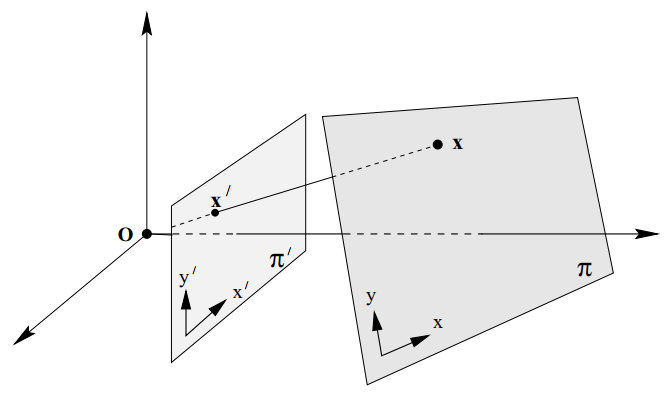
\includegraphics[width=0.7\textwidth]{central_proj.png}
\end{center}
\caption{Central projection maps points from one plane to points on another plane, and also maps lines on one plane to lines on another plane. So there is a projective transformation between corresponding points on these two planes.}
\label{fig:central_proj}
\end{figure}

\begin{figure}[h]
\begin{center}
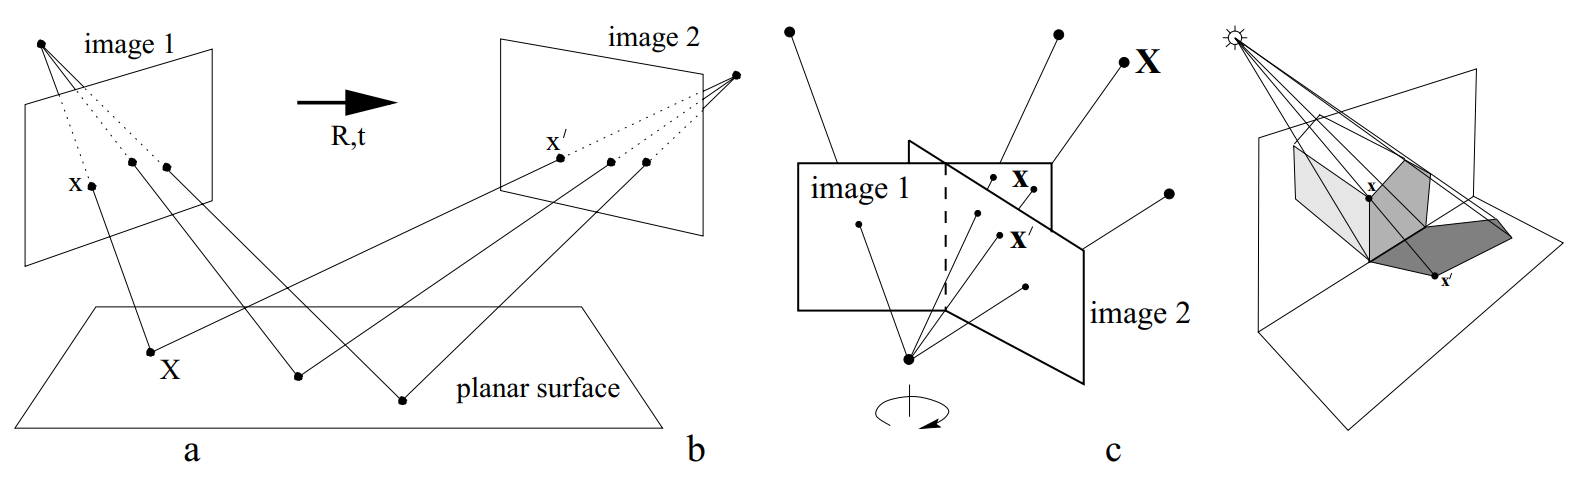
\includegraphics[width=1.0\textwidth]{proj_example.png}
\end{center}
\caption{Examples of a projective transformation. (a) The projective transformation between two images induced by a world space plane (you can easily verify that the \textbf{concatenation} of two
projective transformations is a projective transformation). (b) The projective transformation between
two images with the same camera center (e.g. a camera rotating about its center or a camera varying its focal length); (c) The projective transformation between the image of a plane (the end of the building) and the image of its shadow onto another plane (the ground plane). }
\label{fig:proj_example}
\end{figure}

In camera projection model, the camera center is the projection center and 2D images are projected planes. Therefore, if the camera is only rotating (without translation), then there exist projective transformations between each pair of images (Figure \ref{fig:proj_example}b). Meanwhile, if camera moves but it takes pictures from coplanar points on a global plane surface, then projective transformations also exist between images (Figure \ref{fig:proj_example}a).

Figure \ref{fig:all_proj_example} summarizes all common cases of projective transformation in camera projections. Note that only Figure \ref{fig:all_proj_example}(d) is not projective transformation between the two images while (e) is, since the camera center moves and there exists a projective transformation between two images only if the global points are coplanar.

\begin{figure}[!]
\begin{center}
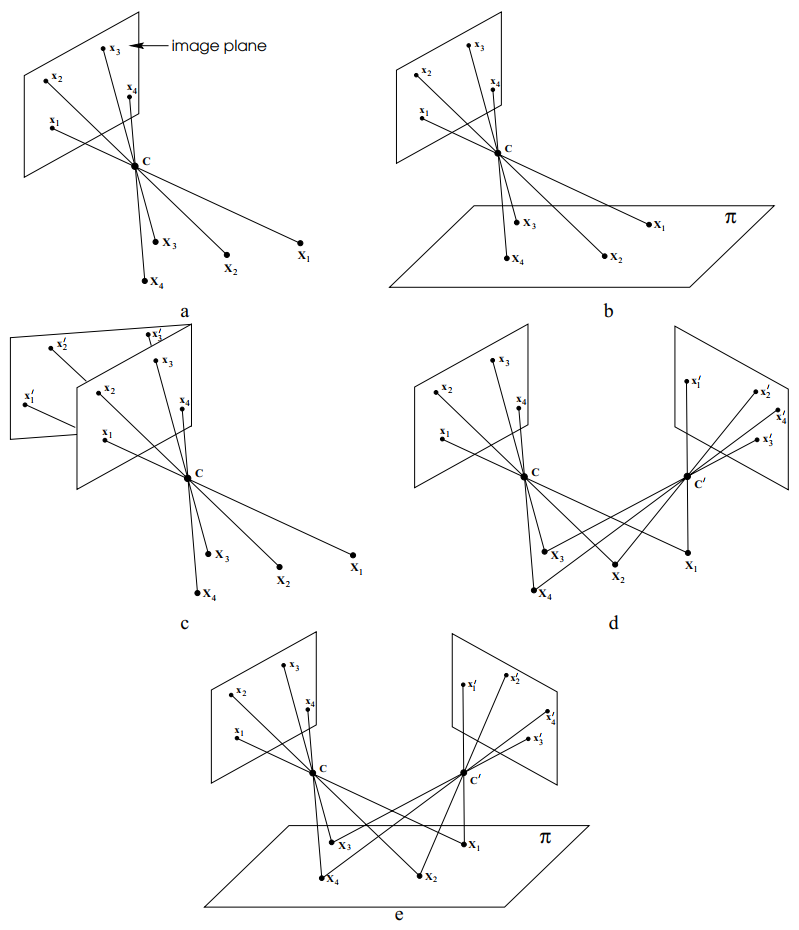
\includegraphics[width=1.0\textwidth]{all_proj.png}
\end{center}
\caption{Different types of camera projections. (a) Image formation. (b) Image and global plane has projective transformation. (c) Two images has projective transformation. (d) Two images do NOT have projective transformation for arbitrary global points. (e) Two images has projective transformation for global coplanar points.}
\label{fig:all_proj_example}
\end{figure}


\subsection{Conics}

In Euclidean geometry, conics are of three main types: hyperbola, ellipse and parabola. A typical conic's equation is $ax^2 + bxy + cy^2 + dx + ey + f = 0$ or in matrix form
\begin{equation}
\mathbf{x^\top C x} = 0
\label{eq:conic}
\end{equation}
where $\mathbf{x} = (x, y, 1)^\top$ in homogeneous format and 
\begin{equation*}
\mathbf{C} = 
\begin{bmatrix}
a & b / 2 & d / 2 \\
b / 2 & c & e / 2 \\
d / 2 & e / 2 & f
\end{bmatrix}
\end{equation*}

The matrix $\mathbf{C}$ is symmetric matrix. We usually use the matrix $\mathbf{C}$ to represent a conic. Note that a conics has 5 degrees of freedom (up to scale) instead of 6. In other words, 5 points determine a conic.

\begin{theorem}
The line $\mathbf{l}$ tangent to a conic $\mathbf{C}$ at a point $\mathbf{x}$ on $\mathbf{C}$ is given by $\mathbf{l} = \mathbf{Cx}$.
\label{theorem:conic}
\end{theorem}
\begin{proof}
Firstly, it is easy to prove that $\mathbf{l}$ passes through $\mathbf{x}$, since $\mathbf{x^\top l = x^\top Cx} = 0$. Next we need to prove $\mathbf{l}$ is tangent to the conic. Suppose $\mathbf{l}$ meets the conic in another point $\mathbf{y}$. Then $\mathbf{y^\top Cy} = 0$ and $\mathbf{ y^\top l = y^\top Cx } = 0 = \mathbf{x^\top Cy }$. Then we have $(\mathbf{x + \alpha y})^\top \mathbf{C} (\mathbf{x + \alpha y}) = 0$ for any scalar value $\alpha$ (you can easily find it true by expanding the equation into terms). That is, the whole line defined by $\mathbf{x, y}$ lies on the conic, which is clearly degenerate (matrix $\mathbf{C}$ is not full rank). Therefore, $\mathbf{l}$ has only 1 intersection point $\mathbf{x}$ on the conic which it is tangent to.
\end{proof}

Note that if $\mathbf{C}$ is not full-rank, then the conic is \textbf{degenerate}, such as two lines $\mathbf{C} = \mathbf{l}_1\mathbf{l}_2^\top + \mathbf{l}_2\mathbf{l}_1^\top$ or a repeated line  $\mathbf{C} = \mathbf{l}\mathbf{l}^\top$.

\subsubsection{Duality and dual conics}
\label{sec:dual_conic}

From the properties of point and lines, we can notice that there is a general duality principal between them. For instance, point on a line is $\mathbf{l^\top x} = \mathbf{x^\top l} = 0$ so their positions can be swapped, so are the situations in Theorem \ref{theorem:line_itsn} and \ref{theorem:point_itsn} which describes the intersection of points and lines. 

A line $\mathbf{l}$ tangent to a point conic $\mathbf{C}$ satisfies $\mathbf{l^\top C^* l} = 0$, where $\mathbf{C}^*$ is the \textit{adjoint matrix} of $\mathbf{C}$. A dual conic is a conic for lines, or a \textbf{line conic}.

We can get $\mathbf{C}^*$ like this: according to Theorem \ref{theorem:conic}, a line tangent to a point conic is $\mathbf{l} = \mathbf{Cx}$, so we have $\mathbf{x} = \mathbf{C^{-1}l}$. Then, $0 = \mathbf{x^\top C x} = \mathbf{l^\top C^{-\top} l} = \mathbf{l^\top C^{-1} l}$. That is, $\mathbf{C}^* = \mathbf{C}^{-1}$ for a non-singular symmetric matrix $\mathbf{C}$.

Note that dual conics are also known as \textbf{conic envelopes}. In geometry, an \textbf{envelope} of a family of curves in the plane is a curve that is tangent to each member of the family at some point, and these points of tangency together form the whole envelope. Therefore, lines satisfying $\mathbf{l^\top C^* l} = 0$ are tangent to point conic $\mathbf{C}$. That is, a point conic $\mathbf{C}$ is the envelope of line family $\mathbf{l}$ (see Figure 2.2 on Page 32 of Ref. \cite{hartley2003multiple}). 

\subsubsection{Transformed conic}
\label{sec:transformed_conic}

\textbf{Transformed point conic}. Under point transformation $\mathbf{x' = Hx}$, we have $0 = \mathbf{x^\top C x} = \mathbf{x'^\top} \mathbf{H}^{-\top}\mathbf{CH}^{-1}\mathbf{x}'$. Therefore, the transformed conic will be $\mathbf{C}' = \mathbf{\mathbf{H}^{-\top}\mathbf{CH}^{-1}}$.

\textbf{Transformed dual conic}. From Section \ref{sec:dual_conic} we know a dual conic (line conic) satisfies $\mathbf{l^\top C^* l} = 0$ with line $\mathbf{l = Cx}$ tangent to original conic $\mathbf{C}$ with tangent point $\mathbf{x}$. And we also know that the transformed line is $\mathbf{l' = H^{-\top}l}$. Then, $\mathbf{l = H^\top l'}$, and further we have $0 = \mathbf{l^\top C^* l} = \mathbf{l'^\top}\mathbf{HC^* H^\top l'}$. Therefore, the transformed dual conic is $\mathbf{C^*}' = \mathbf{HC^{*} H^\top}$.

\subsubsection{The pole$-$polar relationship}

An arbitrary point $\mathbf{x}$ and a point conic $\mathbf{C}$ define a line $\mathbf{l = Cx}$. The line $\mathbf{l}$ is called the \textbf{polar} of $\mathbf{x}$ with respect to $\mathbf{C}$, and point $\mathbf{x}$ is the \textbf{pole} of $\mathbf{l}$ with respect to $\mathbf{C}$. Note that if point $\mathbf{x}$ is on the conic $\mathbf{C}$, then $\mathbf{l}$ is the tangent line of $\mathbf{C}$ at $\mathbf{x}$, which is Theorem \ref{theorem:conic}. \\

\begin{theorem}
The polar line $\mathbf{l = Cx}$ of the point $\mathbf{x}$ with respect to a conic $\mathbf{C}$ intersects the conic in two points. The two lines tangent to $\mathbf{C}$ at these points intersect at $\mathbf{x}$.
\end{theorem}
\begin{proof}
Consider a point $\mathbf{y}$ on $\mathbf{C}$. The tangent line at $\mathbf{y}$ is $\mathbf{Cy}$, and this line contains $\mathbf{x}$ if $\mathbf{x^\top Cy}$ = 0. Using the symmetry of $\mathbf{C}$, the condition $\mathbf{x^\top Cy = (Cx)^\top y} = 0$ is that the point $\mathbf{y}$ lies on the line $\mathbf{Cx}$. Thus the polar line $\mathbf{Cx}$ intersects the conic in the point $\mathbf{y}$ at which the tangent line contains $\mathbf{x}$. 
\end{proof}

Figure \ref{fig:polar_pole} illustrates the polar and pole relationship.

\begin{figure}[h]
\begin{center}
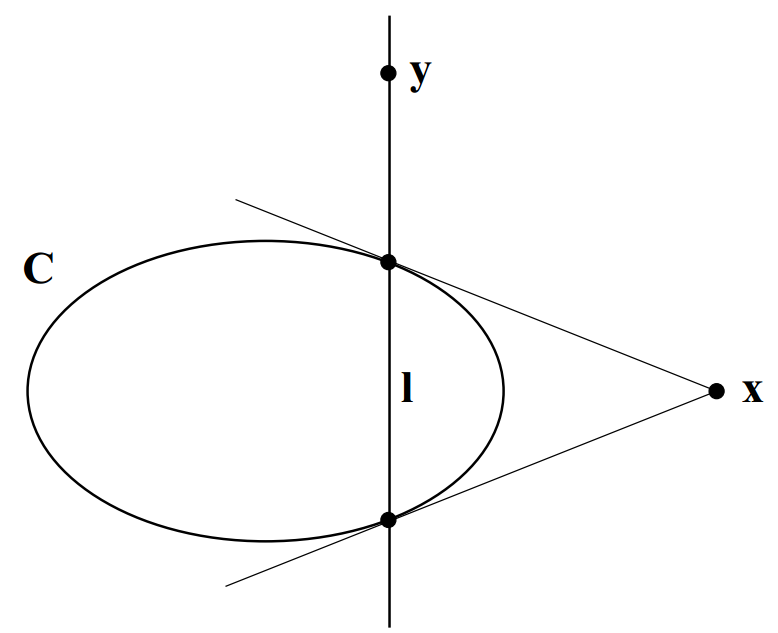
\includegraphics[width=0.5\textwidth]{conic_polar_pole.png}
\end{center}
\caption{Polar and pole relationship.}
\label{fig:polar_pole}
\end{figure}

\subsection{A hierarchy of projective transformations}
\label{2d_proj_trans}

We use $PL(3)$ to denote the group of $3\times 3$ projective transformations. Figure \ref{fig:proj_type} shows common types/subgroups of projective transformations with a hierarchy structure. Each type of transformation group inherits the invariant properties from its upper types. For instance in Figure \ref{fig:proj_type}, the Euclidean transformation on the bottom row has all invariant properties from all types of transformations.

\begin{figure}[h]
\begin{center}
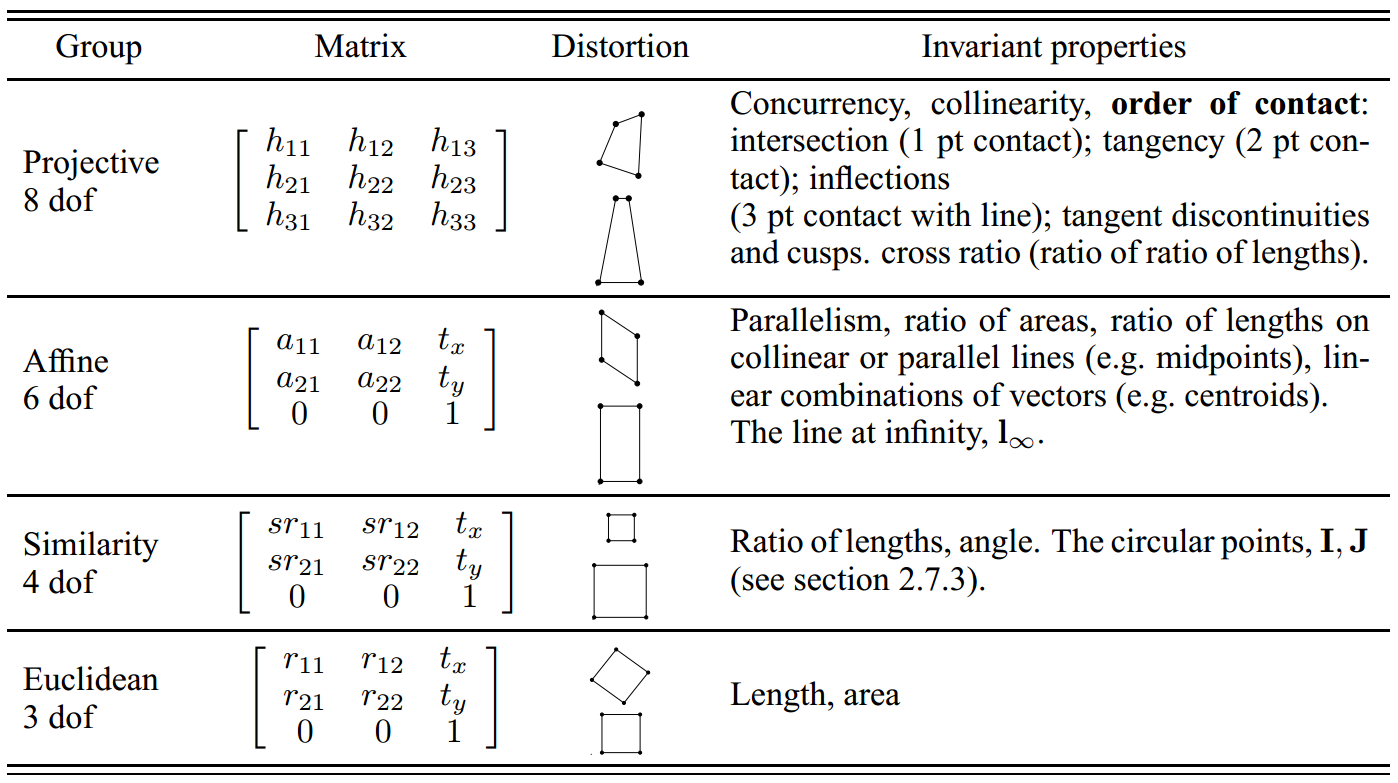
\includegraphics[width=1.0\textwidth]{proj_trans_types.png}
\end{center}
\caption{\textbf{Geometric properties invariant to commonly occurring planar transformations}. The matrix $\mathbf{A}$ is $2\times 2$ matrix, $\mathbf{R}$ is 2D rotation matrix and $t_x, t_y$ is translation. The distortion column shows typical effects of the transformations on a square. }
\label{fig:proj_type}
\end{figure}

\subsubsection{Isometries}

A simple and basic type in $PL(3)$ is isometries which are transformations preserving Euclidean distance. One type of isometry is called \textbf{Euclidean transformation} (or \textbf{rigid transformation}) which is combination of rotation and translation with totally 3 dof:
\begin{equation*}
\mathbf{H_E} = 
\begin{bmatrix}
\mathbf{R} & \mathbf{t} \\
\mathbf{0}^\top & 1
\end{bmatrix}
\end{equation*}

\subsubsection{Similarity transformations}
The next subgroup is \textbf{similarity transformation}, which is an affine matrix with upper left $2\times 2$ part a rotation matrix times a scale factor:
\begin{equation*}
\mathbf{H_S} = 
\begin{bmatrix}
s\mathbf{R} & \mathbf{t} \\
\mathbf{0}^\top & 1
\end{bmatrix}
\end{equation*}
It is the combination of rotation, \textbf{isotropic} scaling and translation with totally 4 dof.

\subsubsection{Affine transformations}

Another subgroup of $PL(3)$ is \textbf{affine transformation} which can be regarded as the combination of rotation, \textbf{anisotropic} scaling and translation. Each affine matrix is a projective transformation matrix with last row $(0, 0, 1)$ like this:
\begin{equation*}
\mathbf{H_A} = 
\begin{bmatrix}
\mathbf{A} & \mathbf{t} \\
\mathbf{0}^\top & 1
\end{bmatrix}
\end{equation*}
Note that according to Singular Value Decomposition (SVD), any non-singular affine matrix can be decomposed into 
\begin{equation*}
\mathbf{A} = \mathbf{UDV} = \mathbf{UV^{-1}VDV} = \mathbf{R(\theta) R(-\phi)DR(\phi)}
\end{equation*}
That is, each affine matrix is the concatenation of a rotation ($R(\phi)$), an anisotropic scaling ($\lambda_1, \lambda_2$ of diagonal matrix $\mathbf{D}$), and a rotation back ($R(\phi)$) and finally another rotation ($R(\theta)$).

\subsubsection{Projective transformations}
\label{sec:proj_trans}
A common projective transformation matrix has 8 degrees of freedom (dof):
\begin{equation*}
\mathbf{H} = 
\begin{bmatrix}
\mathbf{A} & \mathbf{t} \\
\mathbf{v}^\top & 1
\end{bmatrix}
\end{equation*}
with 2 more dof than affine matrix in $\mathbf{v}$, which affects the non-linear effects of the projectivity. Compare the mapping of an ideal point $(x_1, x_2, 0)^\top$ under the two transformations: an affine transformation converts/maps this ideal point to \textbf{another ideal} point $((x_1,x_2)\mathbf{A}^\top, 0)^\top$, while a projective transformation maps the ideal point to a \textbf{finite} point $((x_1,x_2)\mathbf{A}^\top, (x_1,x_2)\mathbf{v})^\top$. Therefore, a projective transformation can model vanishing points.

A projective transformation can be decomposed into a chain of transformations from its subgroups:
\begin{equation}
\mathbf{H} = \mathbf{H_SH_AH_P} =
\begin{bmatrix}
s\mathbf{R} & \mathbf{t} \\
\mathbf{0}^\top & 1
\end{bmatrix}
\begin{bmatrix}
\mathbf{K} & \mathbf{0} \\
\mathbf{0}^\top & 1
\end{bmatrix}
\begin{bmatrix}
\mathbf{I} & \mathbf{0} \\
\mathbf{v}^\top & 1
\end{bmatrix}
=
\begin{bmatrix}
\mathbf{B} & \mathbf{t} \\
\mathbf{v}^\top & 1
\end{bmatrix}
\label{eq:proj_trans_decomp}
\end{equation}
with $\mathbf{B}$ a non-singular matrix given by $\mathbf{B}=s\mathbf{RK} + \mathbf{tv}^\top$, and $\mathbf{K}$ an upper-triangular matrix normalized as $det(\mathbf{K}) = 1$. This decomposition is valid only if $v \neq 0$ and is unique if $s$ is chosen positive. You can easily get this decomposition by running QR decomposition on $\mathbf{B - tv^\top}$. We can see that each decomposed matrix has its own function and does not influence others. Consider the process of rectifying the perspective
image of a global plane (such as example in Figure \ref{fig:central_proj_example}): $\mathbf{H_P}$ (2 dof) moves line at infinity; $\mathbf{H_A}$ (2 dof) affects the affine properties but does not affect lines at infinity; $\mathbf{H_S}$ (4 dof) is general similarity transformation and does not influence affine or projective properties at all. Easily, transformation types in the decomposition in Eq. (\ref{eq:proj_trans_decomp}) can be \textbf{reversed}, i.e., $\mathbf{H}$ can also be decomposed into $\mathbf{H = H_PH_AH_S}$ (of course values in matrices here are different).


\subsection{Remove projective distortion from a perspective image of a global plane}
\label{2d_proj_distortion}

The properties of projective transformation on planes can be used to remove projective distortion from a perspective image of a global plane. Figure \ref{fig:proj_distortion} gives examples of different types of projective distortions in images taken on a global plane.

\begin{figure}[h]
\begin{center}
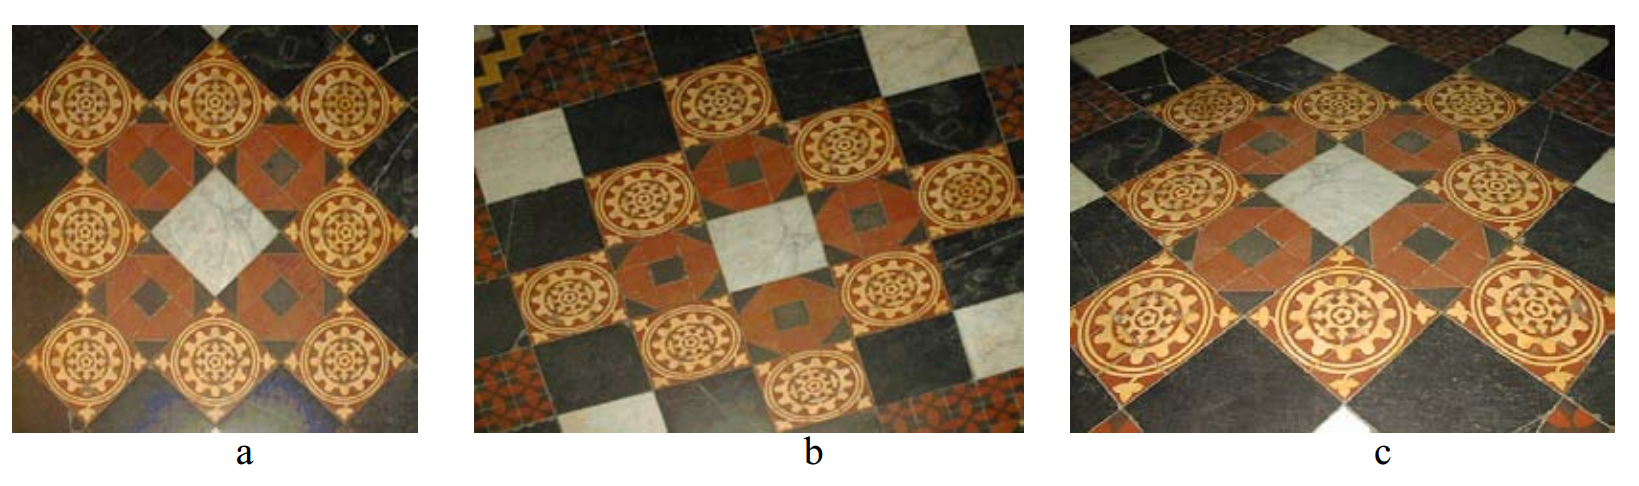
\includegraphics[width=1.0\textwidth]{central_proj_example.png}
\end{center}
\caption{\textbf{Distortions arising under central projection}. (a) Similarity: the
circular pattern is imaged as a circle. A square tile is imaged as a square. Lines which are parallel or perpendicular have the same relative orientation in the image. (b) Affine: The circle is imaged as an ellipse. Orthogonal world lines are not imaged as orthogonal lines. However, the sides of the square tiles, which are parallel in the world are parallel in the image. (c) Projective: Parallel world lines are imaged as converging lines. Tiles closer to the camera have a larger image than those further away.}
\label{fig:proj_distortion}
\end{figure}

There are two common ways to remove projective distortion from an image of a global plane:

\begin{enumerate}
\item The most intuitive way is to explicitly compute the projective transformation between the image plane and global plane, and apply the jtransformation on the image to get the transformed image without distortion (Section \ref{sec:projective_rect} and the second metric rectification method in Section \ref{sec:metric_rect}).
\item Another way is to remove subgroups or `components' of projective transformation one by another. As shown in Eq. (\ref{eq:proj_trans_decomp}), each projective transformation can be decomposed into a chain of transformations from its subgroup $\mathbf{H = H_S H_A H_P}$. Therefore, if we want to measure the affine properties (such as parallelism, ratio of areas) on the original plane from the image, we only need to remove the `projective component' $\mathbf{H_P}$ from $\mathbf{H}$ keep the rest. This process is called \textbf{affine rectification} (Section \ref{sec:affine_rect}). If we want to measure the similarity/metric properties (angles, ratios of lengths) on the original plane from the image, then after removing $\mathbf{H_P}$ in affine rectification, we can further remove the affine component $\mathbf{H_A}$ and leave the similarity transformation only. This is called \textbf{metric rectification} (the first metric rectification method in Section \ref{sec:metric_rect}).
\end{enumerate}

Some important notes about the two above methods:
\begin{enumerate}
\item 
The first method is more straightforward but needs more information to recover the entire projective transformation, while the second way is decomposed into sub-steps and is more flexible in different situations. 
\item
The first method of computing entire projective transformation actually only removes `projective' and `affine' components and still leaves the similarity component (rotation, translation and isotropic scaling), but this doesn't influence further measure, since a similarity transformation almost keeps all important invariant properties (Figure \ref{fig:proj_type}).
\end{enumerate}


\subsubsection{Remove entire projective distortion}
\label{sec:projective_rect}

The most intuitive way for projective rectification is to compute projective transformation directly and apply it onto image to remove entire projective distortion. Each projective transformation $\mathbf{H}$ has 8 dof. Therefore, in order to compute $\mathbf{H}$ between image and global plane, we only need coordinates of \textbf{4 pairs} of point correspondences between image plane and global plane (points must be non-colinear to ensure the coefficient matrix of the 8 equations is full-rank). 

Note that the above method is not applicable to many situations, since we need to get points' coordinates in \textbf{global} plane as input, which are always hard or even impossible to be obtained. Another alternative method only utilizing points from the image will be introduced later in Section \ref{sec:metric_rect}.

\subsubsection{Affine rectification}
\label{sec:affine_rect}

Sometimes we only need to remove the `projective component' from projective transformation in the image and measure affine properties (such as parallelism, ratio of areas) of original global plane from the image. To achieve this, we do not need to recover the entire projective transformation with 8 dof. From the decomposition of projective transformation $\mathbf{H = H_S H_A H_P}$ in Eq. (\ref{eq:proj_trans_decomp}), a `projective component' $\mathbf{H_P}$ only takes 2 dof (in $\mathbf{v}$ on the third row). Therefore, we only need to specify 2 dof in order to determine affine properties. Actually, these 2 dof are given by being associated with the line at infinity $\mathbf{l}_{\infty}$. In this section, we firstly introduce the `invariant factor' under affine transformation, and then describe the affine rectification method based on the invariant factor.

\textbf{Line at infinity and affinity}. As we describe in Section \ref{sec:point_line_infinity}, a line at infinity is denoted as $(0, 0, 1)^\top$. From Section \ref{sec:proj_trans} we know that an affine transformation maps a point at infinity (ideal point) to itself, while a projective transformation maps it to a finite point. This is also the similar to the dual case on line that \textbf{an affine transformation maps a line at infinity to itself}, while a projective transformation maps it to a finite line. To prove this, from Section \ref{sec:trans_line_conic} we know that a 2D line's transformed line is $\mathbf{l}' = \mathbf{H^{-\top}l}$. Then we have:
\begin{equation*}
\mathbf{l}_{\infty}' = \mathbf{H_A^{-\top}l_{\infty}} = 
\begin{bmatrix}
\mathbf{A}^{-\top} & \mathbf{0} \\
\mathbf{-t^\top A^{-\top}} & 1
\end{bmatrix}
\begin{bmatrix}
0 \\
0 \\
1
\end{bmatrix}
=
\begin{bmatrix}
0 \\
0 \\
1
\end{bmatrix}
=
\mathbf{l}_{\infty}
\end{equation*}
The converse is also true, i.e., an affine transformation is the most general linear transformation that fixes $\mathbf{l}_{\infty}$, that is, the vector $\mathbf{v}$ in the third row of transformation matrix must be $\mathbf{0}$. Then we have an important result: \\

\begin{result}
The line at infinity $\mathbf{l}_{\infty}$ is a fixed line under the projective transformation $\mathbf{H}$ \textbf{if and only if} $\mathbf{H}$ is an affinity.
\label{res:affine_fix_infinity}
\end{result}

Note that $\mathbf{l}_{\infty}$ is only fixed linewise but not pointwise. That is, a point at infinity will be mapped by an affinity to another point at infinity instead of itself (unless some special value cases in the affine matrix), even though the line at infinity is still the same.

\textbf{Affine rectification method}. Result \ref{res:affine_fix_infinity} is the core that our affine rectification method refers to. Figure \ref{fig:affine_rect} illustrates the process for affine rectification. In this problem, initially we have the perspective image plane $\pi_2$ (such as Figure \ref{fig:affine_rect_parallelline}a) taken on the global plane $\pi_1$. The line at infinity $\mathbf{l}_{\infty} = (0, 0, 1)^\top$ from global plane $\pi_1$ is mapped to some finite line $\mathbf{l}$ in $\pi_2$. If we can get $\mathbf{l}$ from $\pi_2$, we can compute a transformation $\mathbf{H_P}'$ to transform $\mathbf{l}$ back to $\mathbf{l}_{\infty}$ and get a new transformed image $\pi_3$. Clearly $\mathbf{l}_{\infty}$ is fixed between the global plane and $\pi_3$. Therefore, according to Result \ref{res:affine_fix_infinity}, the transformation between global plane $\pi_1$ and $\pi_3$ must be an affinity. Then, $\pi_3$ is our result image with projective distortion removed (such as Figure \ref{fig:affine_rect_parallelline}b).

\begin{figure}[h]
\begin{center}
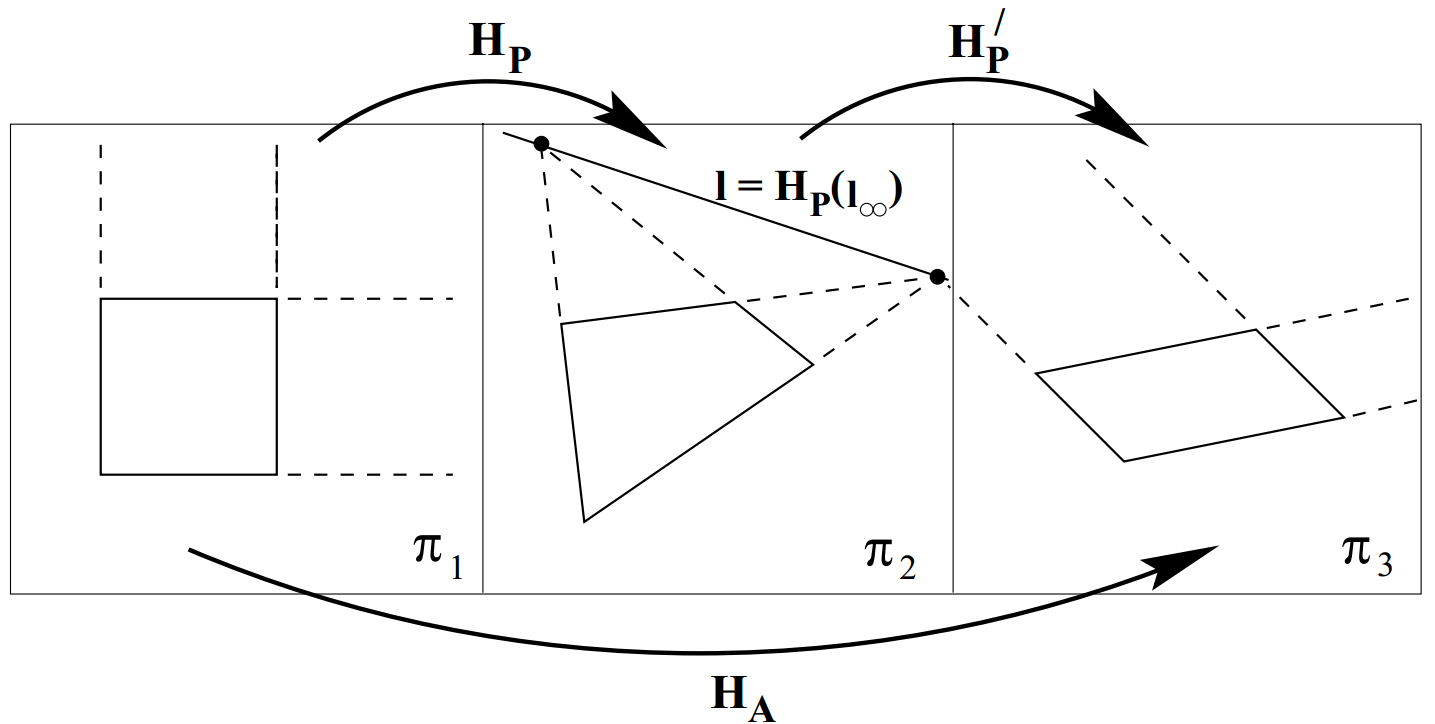
\includegraphics[width=0.8\textwidth]{affine_rect01.png}
\end{center}
\caption{Affine rectification illustration.}
\label{fig:affine_rect}
\end{figure}

Based on the above analysis, we have two sub-problems left: 
\begin{enumerate}
\item How to find the imaged/distorted line at infinity $\mathbf{l}$ in the perspective image? 
\item After we get $\mathbf{l}$, how to compute the new transformation $\mathbf{H_P}'$ to map $\mathbf{l}$ back to $\mathbf{l}_{\infty}$?
\end{enumerate}
Here the second problem is easy to answer. Given $\mathbf{l} = (l_1, l_2, l_3)^\top$ (provided $l_3 \neq 0$), a suitable projective transformation matrix can be
\begin{equation*}
\mathbf{H_P}' = 
\begin{bmatrix}
1 & 0 & 0\\
0 & 1 & 0\\
l_1 & l_2 & l_3
\end{bmatrix}
\end{equation*}

You can easily verify that it transformed $\mathbf{l}$ back to $\mathbf{l}_{\infty}$ since $(\mathbf{H_P}')^{-\top} (l_1, l_2, l_3)^\top = (0, 0, 1)^\top = \mathbf{l}_{\infty}$. 

To solve the first aforementioned problem, we have two common methods:
\begin{enumerate}
\item \textbf{Parallel line method}. In this method, we need to take as input \textbf{2 pairs of lines in the image that are parallel in the global plane}. In order to get the imaged line at infinity, we only need to find two \textbf{vanishing points} (i.e., imaged point at infinity), each of which is actually the imaged point of the intersection of two parallel lines in global plane. This is true based on the property that a projective transformation keeps line intersection. That is, two transformed parallel lines intersects at the transformed intersection point. Figure \ref{fig:affine_rect_parallelline} illustrates this method. We use the 4 lines on the floor as input to find the two intersection points which are vanishing points, and then determine the imaged line at infinity.

\begin{figure}[h]
\begin{center}
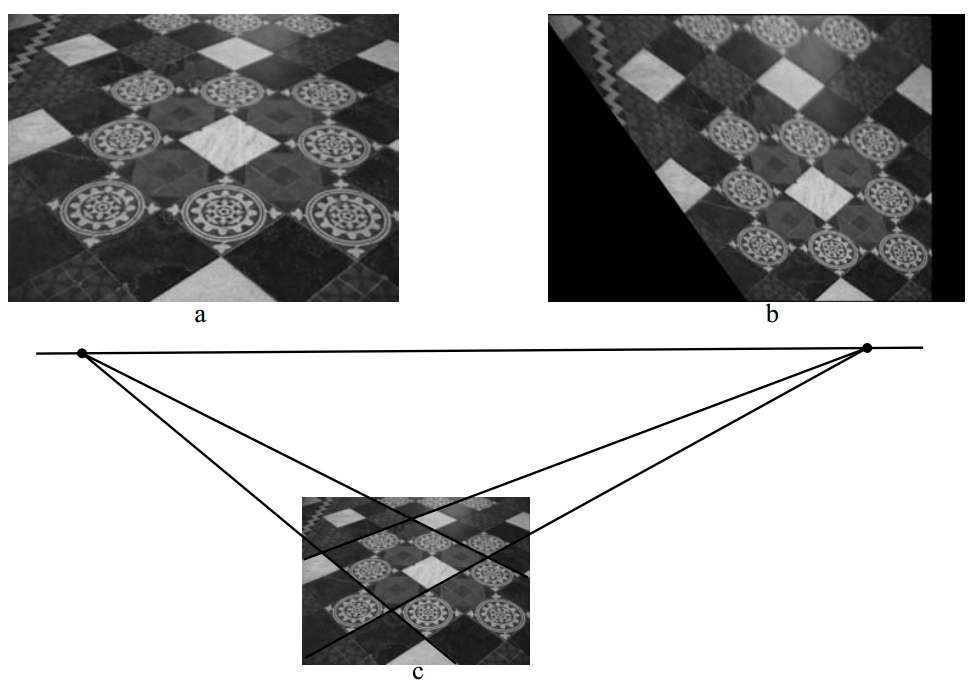
\includegraphics[width=0.8\textwidth]{affine_rect02.png}
\end{center}
\caption{Affine rectification via parallel line method.}
\label{fig:affine_rect_parallelline}
\end{figure}

\item \textbf{Length ratio method}. In this method, we need to take as input \textbf{a pair of 2 intervals on two intersected lines in the image and these intervals' corresponding values in global plane}. The idea of this method is to compute 1D projective transformation $\mathbf{H}_1$ between pairs of points on a imaged line and global line, and then compute the imaged vanishing point using $\mathbf{H}_1$. The input is the ratio of two intervals between three colinear points $\mathbf{a,b,c}$ on the world line and $\mathbf{a',b',c'}$ on the imaged line. Suppose their ratio is $a : b$ on the world line, and $a' : b'$ on the imaged line. So, we can present $\mathbf{a,b,c}$'s 1D coordinates as $(0, 1)^\top, (a, 1)^\top, (a + b, 1)^\top$, and $\mathbf{a',b',c'}$'s coordinates as $(0, 1)^\top, (a', 1)^\top, (a' + b', 1)^\top$. Then, we can use the 3 pairs of corresponding points to compute the 1D projective transformation $\mathbf{H}_1$ between the imaged line and global line, since $\mathbf{H}_1$ is $2\times 2$ matrix with only 3 dof. After this, the vanishing point on the imaged line is $\mathbf{H}_1 (1, 0)^\top$. We can use the same way to get another vanishing point on the other input line, and then the final imaged line at infinity. Figure \ref{fig:affine_rect_lengthratio} illustrates this method.

\begin{figure}[h]
\begin{center}
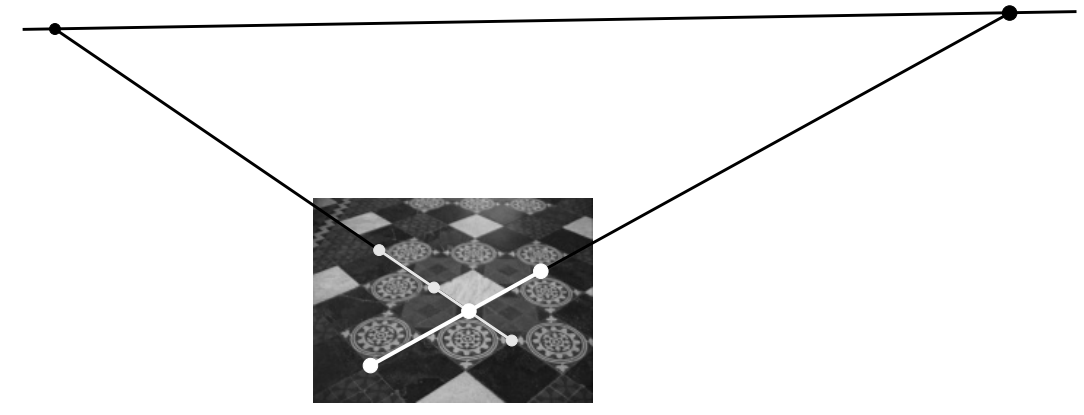
\includegraphics[width=0.8\textwidth]{affine_rect03.png}
\end{center}
\caption{Affine rectification via length ratio method.}
\label{fig:affine_rect_lengthratio}
\end{figure}

\end{enumerate}

\subsubsection{Metric rectification}
\label{sec:metric_rect}

Similar to affine rectification, each projective transformation only has 4 dof more than a similarity transformation, so we only need to specify 4 dof in order to determine metric/similarity properties, or specify 2 more dof based on the result of affine rectification. Similar the the last section, in this section, we firstly introduce the `invariant factor' under similarity transformation, and then describe the metric rectification method based on the invariant factor.

\textbf{1. Circular points and their dual} 

As described in the last section, $\mathbf{l}_{\infty}$ is only fixed linewise but not pointwise by an affinity. However, under any similarity transformation there are two points on $\mathbf{l}_{\infty}$ which are fixed. These are the \textbf{circular points} (also called the \textbf{absolute points}) denoted by $\mathbf{I, J}$, with canonical coordinates 
\begin{equation}
\mathbf{I} = (1, i, 0)^\top, \mathbf{J} = (1, -i, 0)^\top
\label{eq:circular_points}
\end{equation}

The circular points are a pair of complex conjugate ideal points. The name \textbf{circular points} arises because they are the intersection points between a circle and $\mathbf{l}_{\infty}$. By combining their equations
\begin{equation*}
\begin{cases}
& x_1^2 + x_2^2 + dx_1x_3 + ex_2x_3 + fx_3^2 = 0 \\
& \mathbf{l}_{\infty}^\top(x_1, x_2, x_3)^\top = 0
\end{cases}
\end{equation*}
we can get 
\begin{equation}
\begin{cases}
& x_1^2 + x_2^2 = 0 \\
& x_3 = 0
\end{cases}
\label{eq:circular_points_eq}
\end{equation}
whose solution is exactly $\mathbf{I, J}$ in Eq. (\ref{eq:circular_points}), i.e. any circle intersects $\mathbf{l}_{\infty}$ in the circular points.

In Euclidean space, a 2D circle is determined by 3 points, while In general formula Eq. (\ref{eq:conic}), a conic is determined by 5 points, 2 of which is circular points for a circle.

\textbf{2. Circular points are fixed by similarity} 

To see that they are fixed under an orientation-preserving similarity:
\begin{equation}
\mathbf{I}' = \mathbf{H_S I} = 
\begin{bmatrix}
s \cos \theta & -s\sin \theta & t_x \\
s \sin \theta & s\cos \theta & t_y \\
0 & 0 & 1
\end{bmatrix}
\begin{bmatrix}
1\\
i\\
0
\end{bmatrix}
=
s e^{-i\theta} \mathbf{I} = \mathbf{I}
\label{eq:circular_points_fixed}
\end{equation}
since according to Eular's equation, $e^{i\theta} = \cos \theta + i \sin \theta$. Analogous proof is easy for $\mathbf{J}$. The converse is also true and easy to prove. If $\mathbf{H_S I} = s\mathbf{I}$, then $h_{31}, h_{32}$ in the last row must be both 0 and the upper left $2\times 2$ matrix must be a rotation matrix. So we have an important result: \\

\begin{result}
The circular points, $\mathbf{I, J}$ are fixed points under the projective transformation $\mathbf{H}$ \textbf{if and only if} $\mathbf{H}$ is a similarity.
\label{res:circular_points}
\end{result} 


\textbf{3. The conic dual to the circular points}

The dual conic to circular points is 
\begin{equation}
\mathbf{C}_{\infty}^* = \mathbf{IJ^\top + JI^\top},
\label{eq:dual_conic}
\end{equation}
which is a degenerate line conic consisting two circular points. In Euclidean coordinate system we can use $\mathbf{I,J}$'s canonical coordinate in Eq. (\ref{eq:circular_points}) to compute 
\begin{equation}
\mathbf{C}_{\infty}^* = 
\begin{bmatrix}
1 & 0 & 0\\
0 & 1 & 0\\
0 & 0 & 0
\end{bmatrix}.
\label{eq:dual_conic_matrix}
\end{equation}
We can verify that $\mathbf{C}_{\infty}^*$ is fixed under 
transformations in analogous to the fixed properties of circular points $\mathbf{I, J}$, since according to Section \ref{sec:transformed_conic}, the transformed conic is ${\mathbf{C}_{\infty}^{*}}'= \mathbf{H_S}\mathbf{C}_{\infty}\mathbf{H_S}^\top = \mathbf{H_S}(\mathbf{IJ^\top + JI^\top})\mathbf{H_S}^\top = \mathbf{C}_{\infty}$. The converse is also true to be verified. So we have a result similar to the previous one: \\

\begin{result}
The dual conic $\mathbf{C}_{\infty}^*$ is fixed under the projective transformation $\mathbf{H}$ \textbf{if and only if} $\mathbf{H}$ is a similarity.
\label{res:dual_conic}
\end{result}

Note that only under similarity transformation, $\mathbf{I, J}$ are fixed and have canonical coordinates in Eq. (\ref{eq:circular_points}). Under other types of transformation, $\mathbf{I, J}$ are mapped to other points such as finite points. For the dual conic, its general form is Eq. (\ref{eq:dual_conic}) in \textbf{any} coordinate systems, and its special form in Eq. (\ref{eq:dual_conic_matrix}) is only in Euclidean system.

Some properties of $\mathbf{C}_{\infty}^*$: 
\begin{enumerate}
\item $\mathbf{C}_{\infty}^*$ has 4 dof. A $3\times 3$ symmetric matrix has 5 dof, but $\mathbf{C}_{\infty}^*$'s rank is 2, which reduces 1 dof.
\item $\mathbf{l}_{\infty}$ is null vector of $\mathbf{C}_{\infty}^*$. Since $\mathbf{I,J}$ are circular points on $\mathbf{l}_{\infty}$, then $\mathbf{C}_{\infty}^* \mathbf{l}_{\infty} = (\mathbf{IJ^\top + JI^\top})\mathbf{l}_{\infty} = 0$.
\end{enumerate}


\textbf{4. Angle between two lines on the projective plane}

The general format of the angle between two lines $\mathbf{l}$ and $\mathbf{m}$ is
\begin{equation}
\cos \theta = \frac{\mathbf{l^\top C_{\infty}^* m}}{\sqrt{(\mathbf{l^\top C_{\infty}^* l})(\mathbf{m^\top C_{\infty}^* m})}},
\label{eq:2d_line_angle}
\end{equation}
which is the form in any coordinate systems. In the Euclidean system, $\mathbf{C}_{\infty}^*$ is the matrix shown in Eq. (\ref{eq:dual_conic_matrix}), and then the angle between two lines is the common form we are familiar with:
\begin{equation*}
\cos \theta = \frac{\mathbf{l^\top m}}{(\mathbf{l^\top l})(\mathbf{m^\top m})},
\end{equation*}

We can verify that the angle in Eq. (\ref{eq:2d_line_angle}) is invariant to projective transformations, since the transformed numerator in the equation is 
\begin{equation*}
\mathbf{l^\top}' {\mathbf{C}_{\infty}^*}' \mathbf{m}' = (\mathbf{l^\top H^{-1}}) (\mathbf{H}\mathbf{C}_{\infty}^* \mathbf{H}^{\top})(\mathbf{H}^{-\top}\mathbf{m}) = \mathbf{l^\top} {\mathbf{C}_{\infty}^*} \mathbf{m}.
\end{equation*}
Similarly the denominator is also unchanged. Based on Eq. (\ref{eq:2d_line_angle}), we can redefine the orthogonality of two lines with:\\

\begin{result}
Two lines $\mathbf{l, m}$ are orthogonal if $\mathbf{l^\top C_{\infty}^* m} = 0$ in any coordinate system.
\label{res:line_orthogonal}
\end{result}


\textbf{5. Metric rectification method}. 

Review that according to Result \ref{res:affine_fix_infinity}, the affine rectification method transforms the imaged $\mathbf{l}_{\infty}$ to its fixed position to obtain the affine transformation between transformed image and original global plane. Similarly, the metric rectification method here transforms the circular points $\mathbf{I, J}$ to their fixed canonical coordinates in Eq. (\ref{eq:circular_points}). Then, according to Result \ref{res:circular_points}, the transformation between the transformed plane and original global plane must be a similarity. However, in practice instead of transforming $\mathbf{I, J}$, it is easier and more straightforward to follow Result \ref{res:dual_conic} to transform ${\mathbf{C}_{\infty}^*}'$ from the perspective image plane to its original form $\mathbf{C}_{\infty}^*$ in Eq. (\ref{eq:dual_conic_matrix}). Then the transformation between transformed plane and original plane is a similarity.

Using the decomposition chain of each projective transformation, we have
\begin{align}
\begin{split}
{\mathbf{C}_{\infty}^{*}}' &= (\mathbf{H_PH_AH_S})\mathbf{C}_{\infty}(\mathbf{H_PH_AH_S})^\top \\
&= (\mathbf{H_PH_A})(\mathbf{H_S}\mathbf{C}_{\infty}\mathbf{H_S}^\top)(\mathbf{H_PH_A})^\top \\
&= (\mathbf{H_PH_A})\mathbf{C}_{\infty}(\mathbf{H_PH_A})^\top \\
&= 
\begin{bmatrix}
\mathbf{KK^\top} & \mathbf{KK^\top v} \\
\mathbf{v^\top KK^\top} & \mathbf{v^\top KK^\top v}
\end{bmatrix},
\end{split}
\label{eq:conic_decomp}
\end{align}
where $\mathbf{K,v}$ are components of $\mathbf{H_A, H_P}$ shown in Eq. (\ref{eq:proj_trans_decomp}) , respectively. Eq. (\ref{eq:conic_decomp}) shows that the transformed dual conic contains only affine and projective transformation. Therefore, if we can identify ${\mathbf{C}_{\infty}^{*}}'$ in the perspective image, we can compute a transformation $\mathbf{H}$ to transform ${\mathbf{C}_{\infty}^{*}}'$ back to original $\mathbf{C}_{\infty}^{*}$. Clearly, ${\mathbf{C}_{\infty}^{*}}'$ is a symmetric matrix with rank $2$ (its third row is linear representation of the first two rows), so using SVD we can get ${\mathbf{C}_{\infty}^{*}}' = \mathbf{U}\mathbf{C}_{\infty}^{*}\mathbf{U}^\top$, where $\mathbf{C}_{\infty}^{*}$ is the original form in Eq. (\ref{eq:dual_conic_matrix}). Then, $\mathbf{C}_{\infty}^{*} = \mathbf{U}^{-1}{\mathbf{C}_{\infty}^{*}}'\mathbf{U}^{-\top}$, so the final transformation we want is $\mathbf{H} = \mathbf{U}^{-1}$.

Now the only problem left is how to identify ${\mathbf{C}_{\infty}^{*}}'$ in the perspective image. Similar to affine rectification strategy, here we also have two methods:
\begin{enumerate}
\item [(1)]
\textbf{Start from the affinely rectified image plane}. Suppose an image \textbf{has been already affinely rectified}, then we only require two constraints to specify 2 dof in order to determine a metric rectification. The input of this rectification method is two pairs of imaged lines $\mathbf{l', m'}$ which are vertical on the \textbf{global} plane. From Result \ref{res:line_orthogonal}, $\mathbf{l'^\top}{\mathbf{C}_{\infty}^{*}}' \mathbf{m'} = 0$. So using Eq. (\ref{eq:conic_decomp}) with $\mathbf{v = 0}$ (since the image is already affinely rectified so the projective component is gone now), we have
\begin{equation*}
%
\begin{bmatrix}
l_1' & l_2' & l_3'
\end{bmatrix}
%
\begin{bmatrix}
\mathbf{KK^\top} & \mathbf{0}\\
\mathbf{0} & 0
\end{bmatrix}
%
\begin{bmatrix}
m_1'\\
m_2'\\
m_3'
\end{bmatrix}
%
= 0,
\end{equation*}
which is a linear constraint on the $2\times 2$ matrix $\mathbf{S = KK^\top}$ that is symmetric with 2 dof (overall scaling is unimportant). Therefore, two such pairs of vertical lines on the global plane are enough to compute $\mathbf{S}$ and further $\mathbf{K}$ up to scale by Cholesky decomposition. Figure \ref{fig:metric_rect_01} illustrates this method. 

\item [(2)]
\textbf{Compute it from the original perspective image}. If we start from the original image, we need to compute ${\mathbf{C}_{\infty}^{*}}'$ directly. According to previous description, ${\mathbf{C}_{\infty}^{*}}'$ has 4 dof but 1 dof is reduced because it is not full rank, which condition is hard to use during computation. Therefore, we still need to provide 5 constraints. That is, by providing 5 pairs of lines which are vertical on the global plane as input, we can use Result \ref{res:line_orthogonal} to compute ${\mathbf{C}_{\infty}^{*}}'$ linearly. Figure \ref{fig:metric_rect_02} illustrates this method. 
\end{enumerate}


\textbf{Comparison with previous methods}. We have already introduced an intuitive method of computing entire projective transformation in Section \ref{sec:projective_rect}. However, this method takes as input 5 pairs of points from global plane which are very hard to achieve (since we usually only have an image as input and know nothing about the global space). Analogous situation also exists in affine rectification method which needs length ratio from global plane. Compared to them, the metric rectification methods described here only takes as input pairs of lines that are vertical on global plane, which information is much easier to be obtained directly from the image plane (Figure \ref{fig:metric_rect_01}a and \ref{fig:metric_rect_02}a).

\begin{figure}[h]
\begin{center}
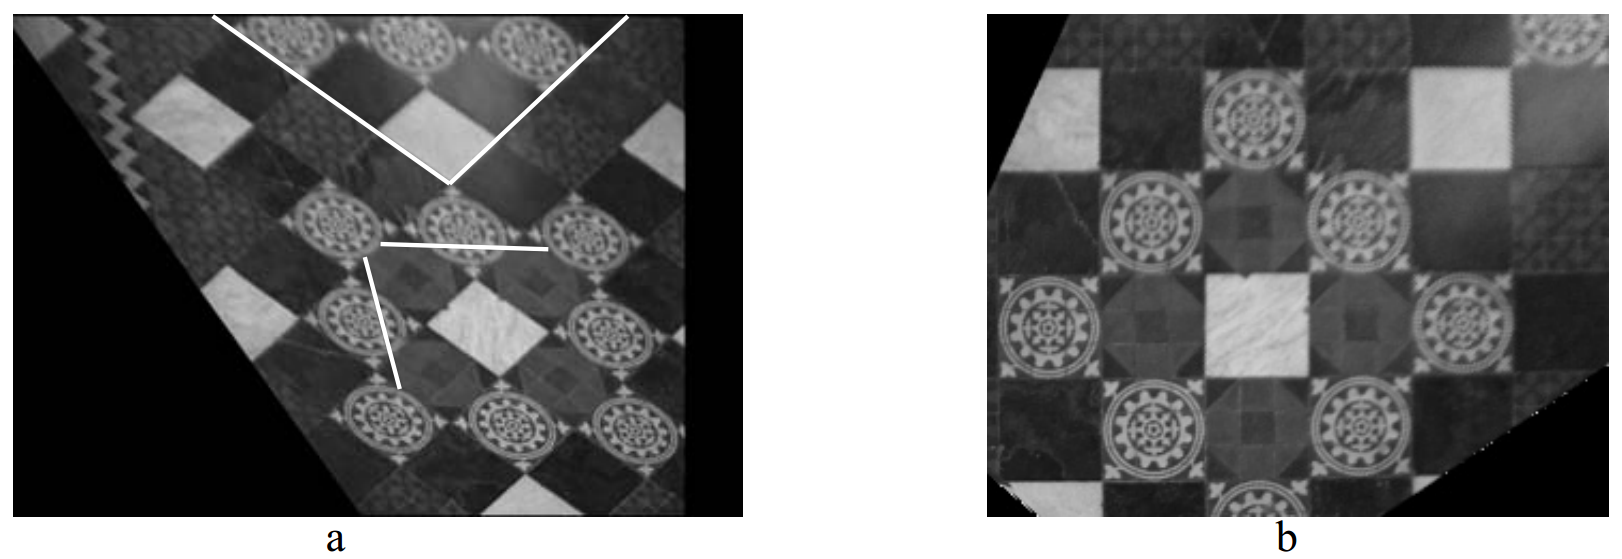
\includegraphics[width=0.8\textwidth]{metric_rect01.png}
\end{center}
\caption{Metric rectification with two pairs of vertical lines from affinely rectified image.}
\label{fig:metric_rect_01}
\end{figure}

\begin{figure}[h]
\begin{center}
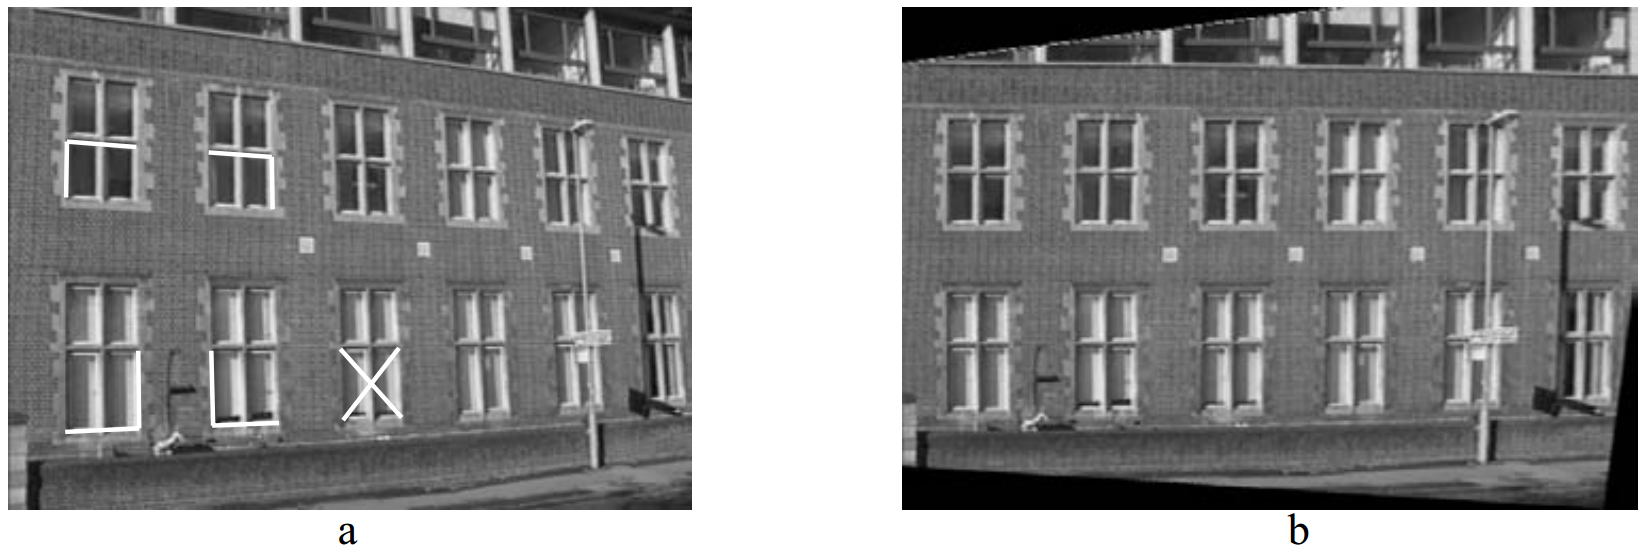
\includegraphics[width=0.8\textwidth]{metric_rect02.png}
\end{center}
\caption{Metric rectification with five pairs of vertical lines from original image.}
\label{fig:metric_rect_02}
\end{figure}

\clearpage

\section{3D projective geometry and transformation}

3D projective geometry and transformation in this section is very analogous to the 2D case in previous Section \ref{sec:2d}. Most of its contents can be regarded as a simple extension from 2D case to 3D.

Similar to $\mathbb{P}^2$ described in Section \ref{sec:2d}, $\mathbb{P}^3$ is equal to $\mathbb{R}^3$ augmented with a set of ideal points which are on the plane $\bm{\pi}_{\infty} = (0, 0, 0, 1)^\top$ (that is, an ideal point is like $(x_1, x_2, x_3, 0)^\top$).


\subsection{3D Points and planes}

A 3D homogeneous point can be written as $\mathbf{X} = (X, Y, Z, 1)^\top$, and a 3D plane can be written as $\bm{\pi} = (\pi_1, \pi_2, \pi_3, \pi_4)$. A point on a plane is written as
\begin{equation}
\bm{\pi}^\top \mathbf{X} = 0.
\end{equation}

We can also use $\mathbf{n^\top \widetilde{X}} + d = 0$, where $\mathbf{n} = (\pi_1, \pi_2, \pi_3)^\top$ is the normal of the plane, $\widetilde{\mathbf{X}} = (X, Y, Z)^\top$ is the inhomogeneous point, and $d = \pi_4$. 

One important property is that, \textbf{3 planes define a point}, and \textbf{3 points define a plane}. That is, plane and point are dual to each other, just like a line and point are dual to each other in the 2D case.

\textbf{Parametrization of point on a plane}. A point $\mathbf{X}$ on a plane $\bm{\pi}$ can be written as $\mathbf{X = Mx}$ where $\mathbf{x}$ is arbitrary 3-vector.

\textbf{Transformation of a plane.} Under a point transformation $\mathbf{x' = HX}$, a plane transforms as 
\begin{equation}
\bm{\pi}' =  \mathbf{H}^{-\top}\bm{\pi},
\end{equation}
since $0 = \bm{\pi}^\top \mathbf{H}^{-1} \mathbf{HX} = \bm{\pi}'\mathbf{x}'$.

\subsection{Quadrics}

A quadric is a surface defined by
\begin{equation}
\mathbf{X^\top Q X} = 0
\label{eq:quadric}
\end{equation}
where $\mathbf{Q}$ is a $4 \times 4$ symmetric matrix. A quadric $\mathbf{Q}$ has 9 dof (10 elements less one for scale).

Properties:
\begin{enumerate}
\item
A quadric defines a polarity between a point and a plane, in a similar manner to the polarity defined by a conic between a point and a line. The plane $\bm{\pi} = \mathbf{QX}$ is the polar plane of $\mathbf{X}$ with respect to $\mathbf{Q}$. Similarly, if  $\mathbf{X}$ is on quadric $\mathbf{Q}$, then plane $\bm{\pi} = \mathbf{QX}$ is the tangent plane to $\mathbf{Q}$ at $\mathbf{X}$.  
\item
The intersection of a plane and a quadric is a conic.
\item
Under a point transformation $\mathbf{X' = HX}$, a  quadric transforms as
\begin{equation}
\mathbf{Q}' = \mathbf{H}^{-\top}\mathbf{QH}^{-1},
\label{eq:quadric_transform}
\end{equation}
since $0 = \mathbf{X^\top Q X} = \mathbf{X}'\mathbf{H}^{-\top} \mathbf{Q} \mathbf{H}^{-1}\mathbf{X}'$.
\item
Analogous to 2D case that the dual of a point conic is line conic, the dual of a 3D point quadric is a \textbf{plane quadric} satisfying $\bm{\pi}^\top \mathbf{Q}^* \bm{\pi} = 0$, where $\mathbf{Q}^* = \mathbf{Q}^{-1}$ if $\mathbf{Q}$ is invertible.

Under a point transformation $\mathbf{X' = HX}$, a dual quadric transforms as
\begin{equation}
{\mathbf{Q}^*}' = \mathbf{H}\mathbf{Q^* H}^{\top},
\label{eq:dual_quadric_transform}
\end{equation}
since $0 = \bm{\pi}^\top \mathbf{Q}^* \bm{\pi} = \bm{\pi}'^\top \mathbf{H}  \mathbf{Q}^* \mathbf{H}^\top \bm{\pi}'$.
\end{enumerate}




\subsection{The hierarchy of 3D Projective transformation}

The properties of 3D transformation can be simply regarded as an extension from 2D transformations (Section \ref{2d_proj_trans}) to 3D. Please refer to Section 3.4 in Ref. \cite{hartley2003multiple} for details.

\subsection{Remove 3D projective distortions}

In Section \ref{2d_proj_distortion}, we described 2D planar projective geometry and distortion removal which identifies three key components: line at infinity $\mathbf{l}_{\infty}$, circular points $\mathbf{I, J}$ on $\mathbf{l}_{\infty}$, and circular points' dual conic $\mathbf{C}_{\infty}^*$. In 3D projective geometry, their corresponding geometric entities are: plane at infinity $\bm{\pi}_{\infty}$, absolute conic $\bm{\Omega}_{\infty}$ on $\bm{\pi}_{\infty}$, and absolute conic's dual quadric $\mathbf{Q}_{\infty}^*$.

\subsubsection{Plane at infinity}

Corresponding to line at infinity $\mathbf{l}_{\infty}$ with canonical position $(0, 0, 1)^\top$ in 2D case, the plane at infinity $\bm{\pi}_{\infty}$ has the canonical position $(0, 0, 0, 1)^\top$ in affine 3-space. It contains the directions $\mathbf{D} = (x_1, x_2, x_3, 0)$, and enables the identification of affine properties such as parallelism: two planes are parallel if and only if their intersection line is on $\bm{\pi}_{\infty}$.

Analogous to $\mathbf{l}_{\infty}$'s property shown Result \ref{res:affine_fix_infinity}, we have similar result for $\bm{\pi}_{\infty}$ that is fixed under 3D affinity: \\

\begin{result}
The plane at infinity, $\bm{\pi}_{\infty}$, is a fixed plane under the projective transformation $\mathbf{H}$ if and only if $\mathbf{H}$ is an affinity.
\label{res:3d_affine_fix_infinity}
\end{result}

The proof is also similar to that of Result \ref{res:affine_fix_infinity}. Also similar to $\mathbf{l}_{\infty}$, $\bm{\pi}_{\infty}$ is only fixed planewise but not pointwise (that is, a point on $\bm{\pi}_{\infty}$ will be transformed to another point on $\bm{\pi}_{\infty}$). 

Section \ref{sec:affine_rect} describes 2D affine rectification which transforms distorted $\mathbf{l}_{\infty}$ to its canonical position and finds the affinely rectified result image w.r.t. Result \ref{res:affine_fix_infinity}. Analogous to this, we can run 3D affine rectification by transforming distorted $\bm{\pi}_{\infty}$ to its canonical position, and then get affinely rectified result w.r.t. Result \ref{res:3d_affine_fix_infinity}.

\subsubsection{Absolute conic}

Corresponding to circular points $\mathbf{I, J}$ on $\mathbf{l}_{\infty}$, the absolute conic $\bm{\Omega}_{\infty}$ is a (point) conic on $\bm{\pi}_{\infty}$. Analogous to circular points' equation in Eq. (\ref{eq:circular_points_eq}), points on $\bm{\Omega}_{\infty}$ satisfy:
\begin{equation}
\begin{cases}
& x_1^2 + x_2^2 + x_3^2 = 0 \\
& x_4 = 0
\end{cases}
\label{eq:absolute_conic_eq}
\end{equation}
which denotes a point conic because the first equation can be presented as
\begin{equation*}
(x_1, x_2, x_3) \mathbf{I} (x_1, x_2, x_3)^\top = 0
\end{equation*}
so that $\bm{\Omega}_{\infty}$ corresponds to a conic $\mathbf{C}$ with matrix $\mathbf{C = I}$. It is thus a conic of \textit{purely imaginary points} on $\bm{\pi}_{\infty}$.

Analogous to circular points $\mathbf{I, J}$ which are fixed under 2D similarity transformation in Result \ref{res:circular_points}, a key property of $\bm{\Omega}_{\infty}$ is that it is a fixed conic under any 3D similarity transformation: \\

\begin{result}
The absolute conic, $\bm{\Omega}_{\infty}$, is a fixed conic under the projective transformation $\mathbf{H}$ \textbf{if and only if} $\mathbf{H}$ is a similarity.
\label{res:absolute_conic}
\end{result}
\begin{proof}
The proof is also similar to that in Result \ref{res:circular_points}. Firstly, since the absolute conic lies in the plane at infinity, a transformation fixing it
must fix the plane at infinity, and hence must be affine. Such a transformation is of the form
\begin{equation*}
\mathbf{H} = 
\begin{bmatrix}
\mathbf{A} & \mathbf{t} \\
\mathbf{0}^\top & 1
\end{bmatrix}
\end{equation*}

Restricting to the plane at infinity, the absolute conic is represented by the matrix $\mathbf{I}_{3\times 3}$. According to Section \ref{sec:transformed_conic}, the transformed conic of is $\mathbf{\mathbf{A}^{-\top}\mathbf{IA}^{-1}} = \mathbf{\mathbf{A}^{-\top}\mathbf{A}^{-1}}$, where $\mathbf{A}$ is the top-left $3 \times 3$ sub-matrix of $\mathbf{H}_{4\times 4}$. Therefore, if $\bm{\Omega}_{\infty}$ is fixed, then $\mathbf{\mathbf{A}^{-\top}\mathbf{A}^{-1}} = \mathbf{I}$, which means $\mathbf{A}^{-1}$ is orthogonal, then $\mathbf{A}$ is a rotation matrix, i.e., $\mathbf{H}$ is similarity. Obviously, the contrary is also correct.
\end{proof}

Similar to 2D line angle defined in Eq. (\ref{eq:2d_line_angle}), we have 3D line angle defined as
\begin{equation}
\cos \theta = \frac{\mathbf{d}_1^\top\bm{\Omega}_{\infty} \mathbf{d}_2}{\sqrt{(\mathbf{d}_1^\top\bm{\Omega}_{\infty} \mathbf{d}_1)(\mathbf{d}_2^\top\bm{\Omega}_{\infty} \mathbf{d}_2)}},
\end{equation}
where $\mathbf{d}_1$ and $\mathbf{d}_2$ are 3D line directions.

\subsubsection{Absolute dual conic}

The dual of the absolute conic $\bm{\Omega}_{\infty}$ is a degenerate dual quadric in 3-space called the absolute dual conic $\mathbf{Q}_{\infty}^*$. Geometrically, $\mathbf{Q}_{\infty}^*$ consists of the \textbf{planes tangent} to $\bm{\Omega}_{\infty}$, so that $\bm{\Omega}_{\infty}$ is the ``rim'' of $\mathbf{Q}_{\infty}^*$. This is called a \textit{rim quadric}. Algebraically, $\mathbf{Q}_{\infty}^*$ is represented by a $4 \times 4$ homogeneous matrix of rank 3, which in metric 3-space has the canonical form 
\begin{equation}
\mathbf{Q}_{\infty}^* = 
\begin{bmatrix}
\mathbf{I} & \mathbf{0} \\
\mathbf{0}^\top & 0
\end{bmatrix}.
\label{eq:absolute_dual_quadric}
\end{equation}
This is analogous to $\mathbf{C}_{\infty}^*$, the dual conic to 2D circular points in Eq. (\ref{eq:dual_conic}).

Section 3.7 (Page 84) in Ref. \cite{hartley2003multiple} shows why 
$\mathbf{Q}_{\infty}^*$ is the set of planes tangent to $\bm{\Omega}_{\infty}$, and also gives another view of the meaning of absolute dual quadric.

Analogous to Result \ref{res:dual_conic}, the absolute dual quadric is fixed under similarity: \\

\begin{result}
The absolute dual quadric, $\mathbf{Q}_{\infty}^*$ is fixed under the projective transformation $\mathbf{H}$ if, and only if, $\mathbf{H}$ is a similarity.
\end{result}
\begin{proof}
The proof is similar to Result \ref{res:dual_conic}. The absolute dual quadric can be fixed if and only if ${\mathbf{Q}_{\infty}^*} = \mathbf{H}\mathbf{Q_{\infty}^* H}^{\top}$ according to Eq. (\ref{eq:dual_quadric_transform}). So, by applying an arbitrary transformation 
\begin{equation*}
\mathbf{H} = 
\begin{bmatrix}
\mathbf{A} & \mathbf{t} \\
\mathbf{v}^\top & k
\end{bmatrix}
\end{equation*} 
and expand the equation, we can ensure that $\mathbf{A}$ is rotation matrix and $\mathbf{v} = \mathbf{0}$. That is, $\mathbf{H}$ is a similarity.
\end{proof}

\begin{result}
The plane at infinity $\bm{\pi}_{\infty}$ is the null-vector of $\mathbf{Q}_{\infty}^*$.
\end{result}

This result holds in any coordinate frame. Firstly when $\mathbf{Q}_{\infty}^*$ has canonical form in Eq. (\ref{eq:absolute_dual_quadric} and $\bm{\pi}_{\infty} = (0, 0, 0, 1)^\top$, clearly $\mathbf{Q}_{\infty}^* \bm{\pi}_{\infty} = \mathbf{0}$. Then, in any frame under point transformation $\mathbf{H}$, we have ${\mathbf{Q}_{\infty}^*}' = \mathbf{H}\mathbf{Q_{\infty}^* H}^{\top}$ and $\bm{\pi}' =  \mathbf{H}^{-\top}\bm{\pi}$, so ${\mathbf{Q}_{\infty}^*}' \bm{\pi}' = \mathbf{H}\mathbf{Q_{\infty}^*} \bm{\pi} = \mathbf{0}$.

Similar to line conic, we have some result related to angle between planes: \\
\begin{result}
The angle between two planes $\bm{\pi}_1$ and $\bm{\pi}_2$ in any frame is given by
\begin{equation}
\cos \theta = \frac{\bm{\pi}_1^\top\mathbf{Q}_{\infty}^* \bm{\pi}_2}{\sqrt{(\bm{\pi}_1^\top\mathbf{Q}_{\infty}^* \bm{\pi}_1)(\bm{\pi}_2^\top\mathbf{Q}_{\infty}^* \bm{\pi}_2)}}
\label{eq:plane_angle}
\end{equation}
\end{result}
The proof is easy by using similar transformation rule of plane and absolute dual quadric. In a Euclidean frame, Eq. (\ref{eq:plane_angle}) is reduced to the common form we know using plane normals. 

\newpage

\bibliographystyle{unsrt}
\bibliography{ref}

\end{document} 